\documentclass{tamuccthesis}
\usepackage[utf8]{inputenc}
\usepackage{float}
\usepackage{fourier} 
\usepackage{array}
\usepackage{makecell}
\usepackage{graphicx}
\usepackage{graphicx}
\usepackage{subcaption}
\usepackage{mwe}
\usepackage{longtable}
\usepackage{amsfonts,amsmath,bm}
\usepackage{amsbsy,natbib}
\usepackage{amsthm}
\usepackage{natbib}
\usepackage{apalike}
\usepackage[vlined,linesnumbered,titlenumbered,algoruled]{algorithm2e}%
\usepackage{listings}
\RequirePackage{graphics,epsf}
\usepackage{setspace}% http://ctan.org/pkg/setspace
% Already loaded by the apa6 documentclass...
\usepackage{etoolbox}% http://ctan.org/pkg/etoolbox



\usepackage[toc,page]{appendix}

\renewcommand{\type}{Thesis}
\renewcommand{\degree}{MASTER OF SCIENCE}	% For thesis
\renewcommand{\major}{Computer Science}	

\begin{document}

\pagenumbering{roman}
%%  Fill in the following information between the brackets
\newcommand{\thesistitle}{First Line of Title\\Second Line of Title}	
\newcommand{\authorsname}{Evan Krell}	
\newcommand{\thesismonth}{December 2018} 
\newcommand{\committeechair}{Dr. Scott A. King}
\newcommand{\committeemembera}{Dr. Luis Garcia}
\newcommand{\committeememberb}{Dr. Alaa Sheta}

% This will create the title and approval page, do not remove
\maketitlepage
\approval

% Put the text of your abstract between the brackets
\theabstract{
Place your abstract here. The text of your abstract must not exceed 350 words.
It should describe your problem, solution and contribution.
}


\tableofcontents
%\pagestyle{headings}  % need this to set up the header
\setlength{\headheight}{36pt}
\listoftables
\listoffigures
\clearpage
\pagestyle{myheadings} 

\pagenumbering{arabic}
\setlength{\headheight}{12pt}

% Chapter 1 
\chapter{Introduction}



\section{Problem Description}

Unmanned surface vehicles have numerous applications for scientific, commercial, and military sectors. They can be used to perform tasks such as towing, shipping, demining, extending communications, target-following, and surveying specified regions. Less concretely, they can serve as remote presence in the marine environment to monitor and analyze the marine environment \cite{manley2008unmanned}. Deployment of humans for continuous or periodic monitoring and exploration consumes a massive amount of time and resources. Unmanned systems can be used to automatically collect substantial data over extended timeframes at a greatly reduced cost. A high degree of marine presence would provide detailed data for insight into the marine environment under a variety of conditions while observing its evolution over time. Such as system benefits ocean modelling, abnormality detection, marine species population estimation, and other oceanographic and marine science concerns. Stationary water and air monitoring stations exist, but the USV's mobility lets it cover vast areas and explore. 

Advances in hardware and robot control systems have lead to the development of highly capable USVs. Miniaturized camera system, compact onboard computers, GPS-based positioning, and autopilot modules have the potential to enable intelligence water surface agents. However, few examples exist of robot boats exhibiting anything more than rudimentary autonomy \cite{bertram2008unmanned}. Many fields are deploying USVs for various purposes, but the missions are highly human-driven. Manual input of waypoints or coverage polygons are the norm for generating USV missions. Obstacle avoidance may be handled by a human on stand-by rather than an automated routine. Today's USVs are largely implemented as tools rather than assigned responsibilities as agents. It is desirable to have an autonomous marine surface agent that has some understanding of its environment and is capable of generating objectives and missions to conduct data-driven investigations to support scientific research goals.

\section{Approach}

This thesis is part of larger research project to create complete autonomous system for USV to act as scientific agents in the marine environment. Since sophisticated guidance and navigation systems are abundant, the focus is on the automatic generation of goals and mission planning to meet those goals. The design of this system is built on the concept of a robot vehicle being operated by multiple distinct intelligent agents, each of which has a specific domain of responsibility. The agents are responsible for setting mission goals, generating mission plans, and executing missions on the vehicle. The system design is described in terms of each agent's role. 

\subsection{Autonomous Agents}

The agents that compose this system are called the Analyst, Surveyor, and Navigator. The Analyst directs the robot's mission by specifying targets and a reward value for each location in the environment (even if that reward is null due to lack of information). The Surveyor generates mission plans in order to fulfill the scientific goals. The missions explicitly attempt to maximize the reward by visiting targets as well as collecting additional, opportunistic rewards when appropriate. Specifically, this means that the Surveyor is aware of both the Analyst's requested targets as well as the reward function that covers the entire environment under study. An example of using both sources for mission planning is to generate a path between two targets that makes minor deviations that increase the reward. Finally, the mission plan is sent to the Navigator who implements the plan on hardware by issuing motor commands that follow the path. A detailed look at the role of each agent follows, as well as a description of their implementation in this thesis. This text presents initial results in a larger research effort to explore the use of these agents to deliver a highly capable autonomous USV for scientific/survey missions. 

\subsubsection{Analyst Agent}

The Analyst most directly relates the system to the goal of implementing an autonomous scientific explorer. Whereas a traditional robot, even one with a high degree of autonomous mobility, has its mission determined by user-specified goals, the Analyst performs data-driven generation of goals for the platform. The Analyst studies available data sources to assign a value of a location's scientific value, or, reward. Over the region that the robot operates, a grid or function is created that maps locations to rewards. Regions, typically polygons, that offer high reward can be specified as targets. This is intended to be analogous to the idea that a human expert can evaluate the relevancy/interest of each location (it may simply be an "I don't know"), but also should be able to select specific areas to survey. The robot should not be tied to a particular Analyst, just as a research vessel should not serve just one client. Though, the hardware and software capabilities may make certain Analyst's goals incompatible with the particular vehicle. A standard format for Analyst's output should be in place to allow multiple Analysts to operate. The defining characteristic of the Analyst is that it uses some data-driven methods to assessing the situation and automatically determining the scientific values. There are numerous approaches to implementing the Analyst, with major features being whether the analysis is online or offline, the use of external data sources, and the mechanisms for determining reward. 

An example of an Analyst is one that uses onboard data streams to learn about its environment and recognize when interesting subjects are available to investigate. This Analyst could be responsible for broad exploration of a particular body of water, such as a bay or lagoon. Unsupervised learning is performed on samples from the robot's onboard camera stream which is used to characterize the environment over time. Particular concepts, or entities, are learned and a general understanding of normality for the region is obtained. The Analyst has certain expectations regarding what it will encounter. A particularly sophisticated Analyst may be associating the learned concepts with times of day, weather conditions, or whatever other relevant information is available. If something unexpected is seen on the mission, the location of the unexpected event is considered to be interesting and its reward is increased. A simple idea for representing interestingness is to classify all observations into fuzzy sets. When a sensor reading gives insufficient weight to a particular set value, or the values are thinly spread across a number of sets, this is proportional to the interestingness of the observation. The updated reward can be assigned to a single cell or group of cells to mark the location as interesting. This can also be set as a specific target, either for consideration in the next mission planning cycle or to interrupt and set a new goal to that target while within a mission. This is an example of an onboard Analyst using both historical data to inform an understanding of the world and online observations to assess potential interesting targets. 

The Analyst need not be involved with machine learning or onboard analysis to be fulfill the role and provide substantial autonomy to a system. What is critical is that data be used to assign reward and select targets. A simpler Analyst that uses occasional updates from internet sources for analysis used in offline mission plan is described next. This Analyst is, for example, interested in collecting data on seagrasses. Every day, a new satellite image is uploaded that captures the water body of interest. The Analyst has studied the history of this imagery. It has some image processing technique for extracting several substrate entities, which include seagrasses. These entities follow the notation $E_{name}$ or $E_{index}$, so that example entities are $E_{sandy}$, $E_{spartina}$, and $E_{5}$. The Analyst can use this data to generate a grid that assigns reward to all cells in the environment. Reward can incorporate multiple characteristics. Consider an uncommon entity $E_{rare}$ that is present is today's image. The presence of $E_{rare}$ gives reward to that cell and those nearby. Consider also a mundane $E_{common}$ that has not been recently surveyed in favour of more interesting entities. To avoid state data and to maintain ongoing observations, the sliding window of entity coverage proportion indicates that $E_{common}$ lacks sufficient data. Thus, reward is given to cells that match that entity's locations. Rather than specific entities, the situation could be that a particular region is seeing unusually fast growth or death of substrates. The speed and acceleration of each substrate can be used to further impact the reward at each cell. In this example, the Analyst is entire offline and only uses the robot's logs to update the coverage counts of each entity. Despite being much less sophisticated than the previous example, this still fulfills the roles of Analyst and is entirely capable of autonomously directing scientific missions. 


\subsubsection{Surveyor Agent}

Given the weighted targets and environment-reward mapping, the Surveyor is responsible for generating a mission to conduct the scientific survey, Mission planning can take on many forms. It is essentially a path planner that handles multiple goals and includes point-to-point and coverage planing. This can be a single path planning module or split into planning subtasks. The all-in-one approach is used in a dynamic programming based path planner where a number of coverage regions and the paths between regions is solved as a single unit. This has optimality advantages since the planning is aware of the entire mission. However, it becomes intractable as the number of nodes to visit increases. Note that the work does not consider terrain, substantially alleviating the computational burden. A basic framework for a mission planner that works with subplans is one where the mission is a sequence of path segments, each either point-to-point (called a \textit{Goto} path in this text) or \textit{Coverage} segment. Path planners dedicated to \textit{Goto} and \textit{Coverage} are invoked by the mission planner. Technically, by this definition a mission planner is itself a form of path planner since the output can reduce to a single mission path. But, here, a mission planner refers to a higher level of planning that calls path planner modules. While the result is a path, the Surveyor has constraints that are incorporated into the mission planning. The Surveyor may have to remove or modify requested targets to ensure that the mission is both feasible and safe. For example, the Analyst may request targets (1, 2, 3), but the Surveyor determines that no feasible mission can accommodate each target. One option is to remove the nodes that make the mission feasible but with the least impact on the mission's reward. Perhaps the solution is (1, 3). Or, the Surveyor may visit each target, but conduct the \textit{Coverage} planner to visit a proportion of each target so that some of each is visited, but less time required for the sampling. In summary, the Surveyor uses mission planning (which calls path planning modules) to create missions that visit targets under optimization and constraint considerations. 

\subsubsection{Navigator Agent}

The Navigator implements mission plans and generates the motor commands that operate the robot. This necessarily occurs online and onboard the vehicle. The agent works directly with hardware, issuing commands and reacting to sensor readings. The typical navigator is a feedback controller using algorithms such as Pure Pursuit for trajectory following and Extended Kalman Filter for state estimation. Also needed is online detection and reaction to problematic situations. The Surveyor can generate plans that are estimated to be feasible and collision-free, but the Navigator uses sensor feedback to ensure the safety of the vehicle and avoid obstacles or other detected dangers. An autonomous vehicle is expected to be working in environments populated by other watercraft, both human and robot-piloted. A sufficiently capable Navigator is aware of and follows marine traffic regulations for safely interacting with other vehicles. While a requirement of any autonomous vehicle, robot navigation is very well developed and is not the focus of this research. The existence of suitable navigation systems is assumed, and the Analyst and Surveyor roles are developed to work with these Navigators. 

\section{Contributions}
\label{section:contributions}

This research has explored the problem of USV autonomy through the development of two collaborating autonomous agents: an Analyst and Surveyor.The Analyst uses (simulated) substrate image data to assign a reward value to each cell in a grid that represents the region that the USV explores. The Analyst uses the grid to find regions that offer a high ratio of reward over area and that facilitate efficient coverage. The Surveyor generates mission plans that visit as many targets as possible, given constraints on the maximum duration and work. Also, the missions take advantage of opportunities where paths can be made to collect additional reward while remaining feasible. Using the system composed of these agents, the research has posed and investigated several research questions as follows. A major contribution of this work is the development of a framework for evaluating techniques to improve the Analyst and Surveyor agents. A second contribution is the implementation of fitness function for metaheuristic path planning that incorporates dynamic water currents and reward. The other contributions are the answers to these questions, as will be discussed in the results. 

Mission planning, in this work, is implemented as selecting a sequence of path planning segments that are planned by invoking an appropriate path planning module. For example, \textit{Goto} planning is handled by a different planner than \textit{Coverage} planning. Rather than exhaustively search all possible missions, each of which requires multiple path planner invocations, can a set of heuristics be used to select a mission that is comparable to that found by exhaustive search?

\begin{itemize}
    \item When using metaheuristic algorithms for \textit{Goto} planning, it has to consider obstacle avoidance, distance minimization, work minimization, and reward maximization. Do the results shown acceptable convergence and repeatibility?

    \item Numerous metaheuristic algorithms exist and have been applied to path planning, though typically only minimizing distance and collisions. Which if these popular algorithms, PSO, GA, DE, or ABC, are best suited to path planning under these conditions?

    \item Can the weights on the significance of work and reward criteria be set to influence the \textit{Goto} path planning toward a desired path behavior? And are the weights that achieve this behavior applicable across multiple situations since it not reasonable to tune them for each path planning task. 

    \item The presence of water currents impact both the Surveyor and Navigator of a USV. A forecast of water currents is expected to impact mission planning, but does periodic updating of the water currents appreciably affect the estimated work? 
\end{itemize}

\section{Prior Work}

Much of the early work in USV research was initiated during WWII by the U.S. Navy, who remains a key player in USV development \cite{bertram2008unmanned}. Military applications include mine-detection, reconnaissance, harbor security, and test targets. Significant growth in USV technology began in the 1990s by the U.S. Navy and continues to this day. A multitude of USVs have been developed outside the military, in academia, commercial, and government \cite{manley2008unmanned} sectors for successful applications in ocean floor mapping, scientific sampling \cite{cokelet2015use}, inspection of industrial platforms, and disaster response \cite{murphy2009robot}. The focus of the proposed research is scientific applications such as benthic mapping and sample collection. While recent advancements in naval USV technology include increasing the autonomy, the scientific use of USVs rarely extends past basic waypoint following or area coverage. The larger goal of this research is mission planning for scientific USV applications, but the target region of interest for this research is narrower. This research is partially motivated by the need to explore the shallow waters along the Texas coast, including inshore bays and lagoons. These regions are of major interest to the local scientific community and it is hoped that the USV and mission planning system developed for this research can be used for practical work in this field. To evaluate the system, a scientific goal is required; seagrasses have been selected as the target due to their ecological importance, interest to local scientific community, and their abundance which ensures that experimentation is always viable. The shallow marine environment introduces unique challenges that influence the design of the boat, as will be discussed. 

As remote sensing systems continue to reduce the human effort in data collection, there is great potential for USVs in oceanographic and marine science applications. A selection of recent examples are as follows. A USV with a sidescan sonar was used in \cite{klemens2017development} for mapping eelgrass in Southern California. A bathymetric map of a lake bed was generated by a USV in \cite{watanabe2016field}. The next example in particular demonstrates the unique character of a USV. The water surface is an air/water interface and is a habitat of specific scientific interest; this region is exactly the operating domain of a USV. A mission is described in \cite{powers2017mobile} where surface temperatures were sampled to produce a high resolution temperature profile of the air/water interface. These example are among many that suggest the growing interest in USVs for scientific applications. 

While numerous successful USV missions have been demonstrated, they have not seen the widespread acceptance of ground and aerial robots. There are several open research problems that impede the proliferation of USVs \cite{bertram2008unmanned}. It is important to remain in contact with deployed USVs in order to make effective use of the remote presence and to respond to emergency situations. The significant cost of over-the-horizon communications for extended USV range is prohibitive to most non-military users. Another issue the logistic complexity of USV deployment and recovery. All but the most shallow-hulled vessels have to exert caution near the shore; some coastal environments may require tedious protocols for deployment of the vehicles. For some tasks, users may find that it is easier to simply use a manned boat or even wade if appropriate. The marine environment is highly corrosive, obstacle-ridden, and subject to sudden and dramatic changes in sea state; these and other factors put USVs at risk and demand reliable and seaworthy vehicles that can survive numerous missions in order to be worth the monetary and logistic cost. There is also a lack of suitable protocols governing USVs that define how they interact with other marine traffic \cite{manley2008unmanned}. Each USV is a stand-alone system whose behavior cannot be reliably predicted by other autonomous vehicles or human ship operators. Finally, the lack of sophisticated autonomy is a major barrier to USV progress. As with other robot modalities, significant attention has been given to autonomous path following control, obstacle detection and avoidance, and path planning. Current USV autonomous systems are largely behavior based and have limited onboard mission planning. Instead, the USVs either perform simple, tedious jobs or are very human-directed \cite{manley2008unmanned}. For example, in a typical survey mission, a USV is given either a set of human-input waypoints or a search region. The USV executes this mission and returns to base where data is then processed offline. Humans are highly involved in all stages of mission execution: setting goals, verifying progress, processing and evaluating results, and re-deploying the vehicle if needed. The vehicle itself has autonomy for mission execution, but mission planning is almost entirely driven by humans. The vehicle is blind in the sense that it executes the mission, but does not consider the safety and feasibility. 

The lack of onboard mission planning severely limits the potential of USVs. It is desirable to have USVs in operation that can be given genera science goals, and that can use local perception, external data sources, and planning algorithms to achieve these goals with minimal human guidance. This is particularly challenging for marine craft as they are subject to dynamic wind and current forces, sudden weather events, tide fluctuation, other water traffic, and obstacles above and below the water surface. These and other factors of the marine environment must be taken into consideration to ensure efficient mission success as well as safety of the vehicle and marine traffic in its vicinity. Some aspects, such as navigational safety and energy efficiency, are largely independent of the autonomous mission. The impact of other aspects, however, is highly dependent on the operating region of a particular application. For example, entanglement with seagrass is significant concern for nearshore operations, but largely negligible further offshore where strong wave action is a major issue. To develop a concrete system that implements mission planning, it is important to have a particular application domain. The proposed research focuses on mission planning for shallow water survey missions. 

Several schemes have been proposed for classification of levels of autonomy in unmanned systems. One such classification scheme describes eleven levels that range from non-autonomous remote control at level 0 to a fully autonomous vehicle at level 10. In a 2017 review of the current state of USV autonomy, the authors conclude that the current overall level of autonomy for USVs is either level 3 or 4 \cite{heo2017case}. According to their classification system, this means that autonomy can be reliably deployed for real-time collision avoidance, detection of environmental changes, and reaction to those changes. The researchers predict that level 10 is decades away. The authors develop a basic set of requirements for a mission planning system suitable for a USV. These can be broadly summarized as two components. First, the USV should be able to assign goals based on available resources. Second, mission re-planning should be performed in reaction to unexpected situations. 

While little research has been done to develop an integrated high-autonomy USV for scientific applications, some progress has been made in military systems. CARACaS is a state-of-the art mission planning system developed by the U.S. Navy for a swarm of unmanned surface vehicles \cite{heo2017case}. This system integrates the vehicle's sensors and software for dynamic mission planning based on the robot's online perception. The major features of the system are as follows. Static obstacles can be detected and avoided. Resources such as available energy are considered when mission planning. Navigation follows COLREGS regulations; these are traffic rules used to avoid collisions between marine vehicles. COLREGS-based navigation has been explored by other researchers, such as in \cite{naeem2012colregs} where the USV always avoided other vehicles by turning starboard. By following these conventions, other boaters following COLREGS are able to coexist safely with the USV. The system also recognizes threats and can adjust the mission to avoid or to pursue foes. CARACaS has a set of basic mission behaviors that can be initiated depending on the situation and goals, such as patrolling an area, tracking targets, monitoring target activity to determine if they pose a threat, and following targets that have been deemed to be suspicious \cite{wolf2017caracas}. Experimental results demonstrated that a fleet of USVs were able to effectively execute multiple tasks over time without human intervention. 

An important step toward greater autonomy, CARACaS demonstrates a high level of adaptive mission planning. However, the system is focused on military application. The current research seeks to develop a system that enables such autonomy for scientific survey and sampling missions. In addition, there are aspects of mission planning that humans routinely rely upon that is not addressed by the mission planning requirements suggested by \cite{heo2017case}. They discuss the importance of maintaining continuous, high resolution perception for onboard detection and response to events. But the use of external updates and forecasts of future events is not addressed, which is a basic component of human mission planning. Consider this situation where a science team is planning to use a boat, whether manned or unmanned, to map some area. In advance, they would be checking the weather to ensure that is reasonable to do so. Even if the boat is robust and not in any danger during, for example, a light storm, the weather conditions could strongly impact the quality of data. An autonomous "science agent" should have some capability to access weather predictions to plan missions that consider both vehicle safety and data quality. It can be argued that accessing these resources will be difficult for a USV where robust communication is still an active research topic. However, the requirement that robots should be continually monitored in order to react to emergencies necessitates that suitable communication exists. 


\chapter{System Design}

The system made up of a number of separate modules, most of which may be run independently. For example, a particular path planner module may be used as a stand-alone program rather than as a part of a larger mission planning program. 

Each of the three intelligent agents previous described are represented by sets of system modules. The Analyst has programs and utilities for determining the reward ("interestingness") of specific targets or cells in the environment's grid representation. It can generate a set of target regions for \textit{Coverage} tasks that will be given to the Surveyor as mission planning goals. The mission generated by the Surveyor is then used by the Pilot who handles the onboard following of the plan as specific motor commands for the robot. This focus of this paper is on the Surveyor's mission planning since it is currently in the best state for meaningful analysis. The Analyst's programs and results will be discussed, but less analysis is done since it currently works with simulated data and optimality is difficult to define.

\section{Implementation of Analyst Agent}

The Analyst implemented in this research is not applied to a specific real-world problem, but rather demonstrates the role's concept on simulated data. The data is a sequence of images, where each color in the image represents an entity and so each cell is associated with a single entity. A completely white cell indicates the absence of an entity, and a black cell indicates that the value is unknown. Only the red value is used for entity assignment, which limits the number of possible entities to 255. The other color values could later be used to represent additional information such as certainty of the identification. (HSV could be used to more intuitively communicate the purpose of the color values; ie: a lower saturated pixel representing less certainty). Since the Analyst needs to assign reward values to all cells in the world representation's grid, an image is a reasonable method for storing entity information. A sequence of images is given to the Analyst, where each image represents a snapshot of the entities at a particular time. A cellular automata is used to perturb the image by adding and remove pixels based on growth and decay rates of each entity type. There are also randomly generated events such as a sudden appearance of some pattern; these represent anomalies that should be noticed by the analyst. 

This example Analyst employs a simple method of reward assignment. The key points is that is uses both the most recent image as well as a recent history in its calculation. Each entity has a weight listed in a table. Here, the table was manually created since the scenario is entirely fabricated. With a sufficiently large history of images, entities could be generated from unsupervised learning and their weight based on some scientific criteria. However, it is assumed that for this example it is either the case that such automatic assessment has taken place or the weights are informed by an expert. There is no requirement that the Analyst is not given some initial human-input information about its environment and goals. It just has to be capable, as a baseline, of automatic reward assignment and target selection. 

The entire environment is segmented into blocks where each block contains a number of cells. The density of entities in each block is used to add reward to each cell in the block. Thus, cells nearby to entities get some reward, proportional to the total strength of weighted entities in that block. The idea is that if the imagery observes something interesting, the area surrounding is also interesting since it may contain unobserved entities or have characteristics that help explain the entities presence. Next, the speed and acceleration of entity growth or decay within that block is calculated and used to add additional reward to the cells. The importance of speed and acceleration of each entity type has its own weight: some entities may have been observed to be fast and this is not interesting. The Analyst records and outputs a separate grid of the reward for each entity type. The total reward of a cell is the summation of the reward in all grids at that cell. Algorithm \ref{alg:reward_assignment} shows this process more concretely. 

In addition to sharing the reward grids with the Surveyor, the Analyst uses them to generate target region intended to be used in \textit{Coverage} planning. A quadtree algorithm is applied on the environment's grid to generate squares that represent coverage areas. Quadtree starts by splitting rectangle into four equally sized sub-rectangles, as shown in Algorithm \ref{alg:quadtree}. It recursively splits each of those rectangles until a base case is reached.
The quadtree enforces a certain maximum grid size in order to not give the Surveyor unreasonable intractable targets. There is also a minimize size because some a useful coverage region has some area to actually cover. The base case of the quadtree algorithm has three opportunities for termination. If the maximum size limit is reached, 90\% of the cells have entities of interest, and there is no terrain present in the region: terminate. If the maximum size limit is reached and it has not yet terminated, this is because there is terrain. Smaller regions with terrain are desired since the strategy for solving coverage paths with terrain present is much more sensitive to the size of the region. The second base case is that the minimum region size is reached: terminate. Terrain is present, but at a more manageable region size. Finally, if the region is at least 90\% terrain, then the region is not worth visiting: terminate. The top $k$ targets are made available to the Surveyor, where $k$ is some arbitrary number that exists since additional targets greatly expand the work computational effort required by the Surveyor. 

While the intention is present an abstract methodology, the Analyst was developed with seagrass studies in mind. Sudden patterns of loss are likely indicators of seagrass bed scarring or other source of damage. Thus, the speed and acceleration of loss can guide the vehicle to investigate. There are also no "fast" seagrasses, so sudden growth would warrant attention. This mentioned is to clarify some of the choices made and to suggest that there is not a single solution to the Analyst implementation. 

\section{Implementation of Surveyor Agent}

\subsection{Environment Representation}


A finite rectangular region is selected as the robot's exploration domain and is divided into a discrete grid of equally sized cells. The resolution impacts the planning quality in two ways. If the cellsize exceeds the diameter of the sensor, then the path planner's coverage estimation differs from reality. Second, more accurate distance, duration, work, and reward estimates are achieved at higher resolutions. Multiple grids are used to represent different characteristics of the environment. The grids used by the Surveyor implemented in this system are listed in Table \ref{tbl:grids}. 

\begin{table}[H]\small
\begin{tabular}{|l|l|}
\hline
Grid          & Description \\
\hline
$G_{region}$    & Binary occupancy grid where 0 indicates free (water) and 1 indicates occupied (terrain) \\
\hline
$G_{magnitude}$ & Cell values are the water current forecast's magnitude for that location \\
\hline
$G_{direction}$ & Cell values are the water current forecast's direction for that location \\
\hline
$G_{reward}$    & Cell values are the reward for that location, as determined by the analyst \\                           
\hline
\end{tabular}
\caption{Descriptions of grids used by the Surveyor to represent the environment.}
\label{tbl:grids}
\end{table}

\subsection{Mission Planning}

A mission planner is a program that takes as input a start location and a number of targets and allowed stop location. The start and stop locations are simply latitude and longitude coordinate points,  but the targets have both coordinate and extent. The coordinate is the center of the region and the extent specifies the area of the region around that point. Collectively, the start, stop, and target locations are called nodes. At the highest level, a solution mission is a sequence of nodes that represents a sequence of mission segments. The mission planners used in this research generate a sequence of \textit{Goto} and \textit{Coverage} path planner segments. A Goto segment is a path from an initial position to a goal position. In this work, the path minimizes distance, work, duration, and maximizes reward. A Coverage segment is a path that generates complete or partial coverage of an area, with respect the resolution of the grid used to represent the space. Complete coverage is ensured by having the cells smaller than the robot's sensor footprint. The goal of the mission planner is visit as many targets as is feasible and end at one of the allowed stop locations.  The mission planner chooses an optimal order in which to visit the targets. Consider a solution mission ( 0, 2, 1, 3 ). This represents a \textit{Goto} path from the start location at node 0 to a target region's entry location at node 2. The entry location is a point on the boundary of a target region that is selected as the point to start from when arriving from a specific previous node. In other words, there may be a different entry point into the region of node 2 if the previous node were 1 rather than 0. At node 2, the \textit{Coverage} path is performed by visiting cells in the region and ending at the region's exit location. Similarly to the entry location, the exit location is defined with respect to the next node in the sequence. This is illustrated in Figure \ref{segment_example}. After completing the \textit{Coverage} task, another \textit{Goto} task is followed to reach the entry location for node 1. Again, a \textit{Coverage} task is done followed by a \textit{Goto} to reach the stop at node 3. The output of the mission planner should be a feasible path, which is one whose total duration and work do not exceed the maximum constraints. For example, the robot may have both limited power and a directive to end within 5 hours. The mission planner produces only estimates of feasible paths, but will be considered feasible for the purpose of this analysis. Concerns regarding the estimated versus actual feasibility of a path is discussed later. 

\begin{figure}[h]
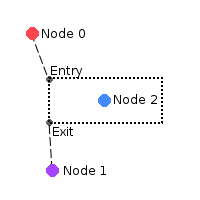
\includegraphics[]{segment_example.png}
\caption{An example mission planning segment. The entry and exit locations for a node's region are dependent on the previous and next nodes in sequence.}
\label{segment_example}
\end{figure}

Two mission planner programs have been developed and their results will be compared in this text. These are called Mission Planner Fully Connected (MPFC) and Mission Planner Try \& Repair (MPTR), and they largely differ in the number of path planner modules invoked. Ultimately, mission planning reduces to a form of the travelling salesman problem which is NP-hard. Various techniques have been developed to deal with NP-hard problems by reducing the search space with heuristics or meta-heuristic approaches. An example is A* which uses the distance between nodes as a heuristic in deciding which nodes to explore. Meta-heuristic algorithms, such as those used by planning modules in this system, have been demonstrated to achieve very high computational performance in reaching (non-deterministic) approximately optimal solutions. Because this system uses different types of search algorithms in different module, a distinction needs to be clarified to avoid confusion. Both mission planners invoke path planners for finding specific paths for each mission segment. Only the selection of targets and the order of these segments is handled by the mission planner itself. MPFC is an exhaustive search of all possible paths. The estimated distance, duration, work, and reward is totalled for each possibility and used to select the best feasible mission. This called optimal with respect to all other missions, but cannot be called absolutely optimal with regards to the path since the segments are computed using approximately optimal path planners. Optimally here is intended to convey an ideal mission planning result given the mission planning setup in place. The point is to compare to the result MPTR which uses heuristics to limit the search space. It generates fewer (in the best case, only one) mission. Thus, the number of path invocations is dramatically lower than that of MPFC. The overwhelming bulk of computing is done in these path planners, so MPRT has potential to reduce the mission planning to minutes instead of hours. Both MPFC and MPRT will now be discussed in full.

\subsection{Mission Planning Inputs}

The required data files for both mission planners are listed in Table \ref{tbl:planner_input}. The table describes each input file and lists where an example of the file can be found in this text. 


\begin{table}[H]\small
\begin{tabular}{|p{2.75cm}|p{5cm}|l|l|}
\hline
Name & Description & File type & Example in text \\
\hline
System config    & Numerous system parameters  & YaML (plaintext) & Appendix listing \ref{lst:system_config} \\
\hline
Entities config  & Weights, labels, and color codes for entities  & YaML (plaintext) & Appendix listing \ref{lst:entities_config}  \\
\hline
Targets table    & Targets to include in mission planning & CSV (plaintext)  & Table \ref{tbl:targets} \\
\hline
Safepoints table & Choices of robot end points & CSV (plaintext)  & Table \ref{tbl:safepoints} \\
\hline
Region map       & Occupancy grid where cells are either occupied or free  & Geotiff raster & Figure \ref{fig:env_terrain} \\
\hline
Water currents magnitude & Grid of predicted magnitudes, 1 band per interval  & Geotiff raster & Figure \ref{fig:currents_intervals} \\
\hline
Water currents direction & Grid of predicted directions, 1 band per interval & Geotiff raster & Figure \ref{fig:currents_intervals} \\
\hline
Entities map & An image where entities are represented by colors. & PNG image & Figure \ref{fig:env_entities} \\
\hline
Entity analysis  & Cell is the Analyst's information on that cell. Bands for entity density, speed, and acceleration scores. & Geotiff raster  &  \\ 
\hline
\end{tabular}
\caption{Input files required for mission planning}
\label{tbl:planner_input}

\end{table}


\subsection{Mission Planner Fully Connected (MPFC)}

MPFC exhaustively searches all possible missions (sequences of path segments) given a start node, set of target nodes, and set of allowed stop nodes. It calls a PSO-based meta-heuristic planner for \textit{Goto} paths and calls a \textit{Coverage} planner that selects between two planning schemes depending on the presence or absence of terrain in the coverage region. A simple lawnmower (row-wise or colwise-wise movement) is chosen in the absence of terrain, and a GA-based planner otherwise. For every possible path, each planning segment is performed. Every path's result and metrics are stored to disc. Once every mission has been computed, the maximum work and maximum duration constraints are applied to filter out infeasible missions. Of the remaining, feasible, missions, the one with highest reward is selected as the top, or relatively optimal, mission. This is based on the idea that, since the vehicle's goal is to collect reward, higher reward is priority over duration and work. The duration and work has been optimized within the individual path planners and then used to remove infeasible missions. Since all feasible solutions are output, further processing could be done to select based on some criteria. For example, the highest-reward mission on the solution's pareto front.

Unfortunately, opportunities for dynamic programming are limited. Each planning segment is dependent on having an estimate of the duration that has elapsed during the previous segments so that it can access the current time interval for the dynamic water currents forecast. Also, the paths are not between the nodes, but to and from entry and exit locations as previously discussed as demonstrated in Figure \ref{segment_example}. Memoization may occur for a paths "prefix", or, the sequence of previous segments minus the immediate previous. The specific case of the non-applicability of the immediate previous is that it may be a \textit{Coverage} segment whose stop point depends on the current node. If these restrictions were removed, the situation would be quite different. The mission planner could simply perform each \textit{Coverage} task and then the \textit{Goto} between each node. Enumerating the possible missions would be a simple table lookup for each estimated metric, totalling them for mission metrics. This motivates the question of to what extent does the water current's dynamism impact the mission planning. If a single water current snapshot could be used, it would allow much more solution reuse. 



%-------------- Mission Planner Try & Repair -----
\begin{algorithm}%
\KwIn{Robot start coordinates $S$, \\
~~~~~~Targets table $T_{targets}$, Safepoints table $T_{safe}$, \\
~~~~~~Maximum duration $D_{max}$, Maximum work $W_{max}$       \\
}
\KwOut{Selected mission $m_{top}$, feasible missions $M_{feasible}$, infeasible missions $M_{infeasible}$}
\textbf{Begin Mission Planner Fully-Connected}\\
~~~Create table $T_{region2point}$, gives the closest point in coverage region to another point (see Figure \ref{segment_example}) \\
~~~Initialize empty list of feasible missions $M_{feasible}$ \\
~~~Intiialize empty list of infeasible missions $M_{infeasible}$ \\
~~~Create list $P$ of possible mission node combos \tcp{Each is start node, a combo of targets $\in T_{targets}$, and a safepoint $\in T_{safe}$}
~~~Update each mission $p \in P$ using $T_{region2point}$ to get the start and end points of each mission segment
~~~\textbf{For} each mission $p \in P$ \\
~~~~~~~Duration $d$ = 0 \\
~~~~~~~\textbf{For} each consecutive pair of nodes $P_i, P_j$ \\ 
~~~~~~~~~~~Invoke \textit{Goto} planner: $P_i \rightarrow P_j$ (Apply offset $d$) \\
~~~~~~~~~~~Update $d$ with estimated duration elapsed in \textit{Goto} \\
~~~~~~~~~~~Invoke \textit{Coverage}: Region $P_j$ (Apply offset $d$) \\
~~~~~~~~~~~Update $d$ with estimated duration elapsed in \textit{Coverage} \\
~~~~~~~Calculate total work $w$ from the results of each segment \\
~~~~~~~\textbf{If} $d$ < $D_{max}$ and $w$ < $W_{max}$ \\
~~~~~~~~~~~Append $p$ to $M_{feasible}$ \\
~~~~~~~\textbf{Else} \\
~~~~~~~~~~~Append $p$ to $M_{infeasible}$ \\
~~~~Sort (descending) $M_{feasible}$ by duration, work, then reward \\
~~~~Set $m_{top}$ as first element in $M_{feasible}$ \tcp{Feasible with highest reward}
\textbf{End Mission Planner Fully-Connected}\\
\caption{Mission Planner Fully-Connected}
\label{alg:MPFC}
\end{algorithm}

\subsection{Mission Planner Try \& Repair (MPTC)}

This system is not built with the MPFC in mind. It exists only to have a relative optimal mission in order to compare to the result of MPTR. Like MPFC, MPTR enumerates every possible mission, but with a critical distinction that greatly impacts the computational cost. Where MPFC calls path planners for each path segment, MPTR calculates a set of scores in place of \textit{Goto} and \textit{Coverage} planners. These scores are combined into a single fitness value for that mission. MPTR does not use the elapsed duration when calculating these scores, which enables greater memoization. 

An overview of MPTR is given in Algorithm \ref{__}. After assigning a total fitness for each possible mission, the missions are filtered on the basis of their estimated duration. The duration is estimated from the straight-line distance between nodes and the distance in traversing the coverage task regions. Since these distances are not based on the actual paths (those will be generated after selecting the mission), the duration is a very rough estimate intended to avoid path planning for missions that are unlikely or impossible to be feasible. In most cases, the duration will be a appreciably higher than this estimate because the actual paths will navigate through the environment in various ways: avoiding obstacles, water currents, and collecting opportunistic reward. There is a possibility, presumably slight, that a \textit{Coverage} task has so much terrain that the vehicle only visits a small fraction of the target region. The overestimate is expected to be a rare case. Currently, the maximum duration is reduced by ten percent to filter more infeasible missions, at the risk of some loss of good solutions. In the trials conducted, ten percent reduction only removed infeasible missions. After filtering, the top mission is selected based on the highest fitness value. The mission is now evaluated in full, computing both \textit{Goto} and \textit{Coverage} paths. Because the node sequence in this mission was selected using heuristics and sampling, it is possible that the mission is found to be infeasible once fully expanded. In this case, the path undergoes a repair process. 

The repair process has two phases, \textit{unlink} followed by \textit{link}. In the \textit{unlink} phase, mission segments are selected for removal based on their impact on the reward. A pivot set is a set of nodes to remove from a mission, and a minimum pivot set is one that causes the remaining duration and work to be feasible with minimum negative impact on the mission reward. The FindPivots algorithm is shown in Algorithm \ref{____}. The pivots are removed (unlinked) and the mission is connected again with the \textit{link} phase. The mission preceding the first pivot may be re-used since the duration is unaffected, but the remaining segments require re-planning. This process is repeated until a feasible mission is found. 

The expectation is the submissions of highly fit missions will also be of high quality. Therefore, fixing a mission that (if the heuristic methods work as intended) barely exceeds the constraints will produce a good mission. Another approach would be to immediately evaluate the next-best mission. Two considerations led to the rejection of this approach. First, other missions with similar fitness are so because they cover the same amount of targets: the order is different. It is probably that such a mission will be another infeasible solution and in an undesired order. The culprit segment could be a \textit{Coverage} or \textit{Goto} task that is present in most or all of the missions of nearby fitness. A more direct approach is to find and remove the problematic segments. While possibly choosing suboptimally, this direct approach will be more efficient than verifying potentially a large number of missions. Consider a case where three smaller \textit{Coverage} tasks form a minimum pivot set. To discover that these three nodes should be removed by exhaustively evaluating the next-highest-fit mission would take significant computation. Because additional nodes increase reward, all those where only one of the three would be checked before those with two, and finally with three. Depending on the effectiveness of the heuristics, it returns to much that same problem as the fully connected planner. Perfecting the heuristics will be difficult because of the breadth of possible scenarios and environments and the limitations of sampling-based estimates for dynamic systems. Therefore, the try and repair approach is adopted to reduce computational effort in the presence of imperfect heuristics. 

%-------------- Mission Planner Try & Repair -----
\begin{algorithm}%

\caption{MPTR} 
\label{alg:MPTR}
\end{algorithm}

%-------------------- Find Pivots ---------------
\begin{algorithm}%
\KwIn{path nodes $N$, \\
~~~~~~path duration segments $D$, \\
~~~~~~path work segments $W$, \\
~~~~~~duration maximum $d$, \\ 
~~~~~~work maximum $w$, \\
}
\KwOut{Solution $P$} \\
\textbf{Begin FindPivots}\\
~~~Initialize empty list of pivot sets $P$ \\
~~~\textbf{If} sum($D$) < $d$ and sum($W$) < $w$ \\
~~~~~~~Return $P$ \\
~~~\textbf{For} each combination $C$ of the nodes $N$ \\
~~~~~~~\textbf{If} sum($D$) - sum($w_i$ \forall $i$ \in $C$) < $d$ \\
~~~~~~~~~~~and sum($W$) - sum($w_i$ \forall $i$ \in $C$) < $w$ \\
~~~~~~~~~~~Append $C$ to list of pivot sets $P$ \\
~~~\textbf{For} pivot set $p_i$ in $P$ \\
~~~~~~~\textbf{For} pivot set $p_j$ in $P$ \\
~~~~~~~~~~~~\textbf{If} $p_i \subset p_j$ \\
~~~~~~~~~~~~~~~~Remove $p_i$ from $P$ \\
\textbf{End FindPivots}\\
\caption{FindPivots} 
\label{alg:find_pivots}
\end{algorithm}
%---------------- End Find Pivots --------------

\section{Path Planning}

\subsection{Goto Path Planner}
\label{section:goto}
The \textit{Goto} planning module is responsible for generating point-to-point paths between a start and stop location. The module is used by the mission planners to plan mission segments between nodes (targets, start, and stop locations). Due to the complexity of path planning (NP-hard), heuristic and meta-heuristic algorithms have become standard approaches rather than optimal methods such as breadth-first search which enumerates all possible paths. Because the scientific missions are expected to operate over very large areas, the search space will be massive. This motivates the emphasis on meta-heuristic algorithms that dramatically reduce the search space at the expense of some optimality. The experiments in this text use a 1000x1093 grid which is very large for planning, could still be called low resolution for the 229,622,675.423 $m^2$ region. The actual grid size for real mission should be such that the sensor covers a cell entirely if complete coverage is required. As discussed in the \ref{lit_review}, meta-heuristic path planning is well-established to give approximately optimal results in point-to-point planning that minimizes distance, duration and avoids obstacles. Rather than repeat this known result, the investigation here focuses on a comparison of algorithms and the effect of including the criteria of minimizing work and maximizing reward. Does one algorithm perform better than the others and is this affected by the addition of work and reward optimization? Can the weights be manipulated to achieved a desired planning behavior that is reliable across multiple situations? Four common meta-hueristic algorithms are compared to select the best to be the \textit{Goto} planner's default algorithm: GA, DE, PSO, and BEE. All four are implemented using the PyGMO optimization library. 

\subsubsection{Genetic Algorithm}

GA is based on the evolutionary concept of natural selection to iteratively evolve toward an optimal solution. The core of GA is that survival of the fittest is used to transform a population of individuals, each a potential solution, into another population with higher average fitness. After evolution proceeds for some time, the fitness should become stable: the fitness of the population is approximately (possibly local) optimum and receive little or no benefit from additional iterations. The individual with highest fitness is chosen as the problem solution. The mechanisms behind GA are the selection, mutation, and crossover operations. Selection is process of choosing which individual's solutions are to be used for constructing the next generation. Individuals are ranked by their fitness and the probability of selection is proportional to the individual's fitness. New individuals are formed from those selected using crossover and mutation. The crossover operation combines elements of solutions (called genes) in combination, with the hope that elements from two fit solutions can be combined to yield an even better solution. While not all of these combinations will have better fitness, the selection process will favor the better results: guiding the population in increasingly fitter solutions on average. Mutation is the operation of randomly adding, deleting, and transforming genes. Many mutations will be harmful, but again, selection will promote the survival of those that improve the population. The result of GA is sensitive to the rate of mutation and crossover. An overemphasis on crossover may lead to premature convergence to an optimal solution, since the space is insufficiently explores. But an overemphasis of mutation may not take advantage of fit solutions and delay convergence. An overview of the GA process is in Algorithm \ref{GA}.

% --------------------  Genetic Algorithm --------------      
\begin{algorithm}%
\KwIn{population size $P$, \\
~~~~~~number of iterations $N$, \\
~~~~~~mutation rate $M$, \\
~~~~~~crossover rate $C$, \\
}
\KwOut{Solution $X$}
\textbf{begin GA}\\
~~~Randomly initialize a population of $P$ individuals\\
~~~Set iteration counter $c$ = 0 \\
~~~\textbf{While} (While $c$ is less than $I$) do\\
~~~~~~~~~~~\textbf{For} i = 1 to number of individuals \\
 ~~~~~~~~~~~~~Evaluate the fitness:= $ f(x_i)$\\
 ~~~~~~~~~~~~~Select individuals with probability proportional to their fitness \\
 ~~~~~~~~~~~~~Apply crossover to selected individuals with probability $C$\\
 ~~~~~~~~~~~~~Apply mutation to selected individuals with probability $M$ \\
 ~~~~~~~~~~~~~Set the current solution $X$ as the fittest individual \\
 ~~~~~~~~~~~~~Set the population as the resulting generation from application of the genetic operations\\
~~~\textbf{End while} \\
\textbf{end GA}\\
\caption{Basic steps of GA}
\label{GA}
\end{algorithm}
% ----------------- End Genetic Algorithm --------------

\subsubsection{Particle Swarm Optimization}

PSO differs conceptually from GA in that it deals with activity within a single, static population, rather than its evolution. The algorithm models a group of social particle, each a solution, that share information to locate resources. They search for resources within the problem's search space, using a fitness function to determine which points offer better resources. Particle are characterized by their positions (solutions), its personal best solution, and its velocity. Each also has access to the global best solution. At every iteration, particle move in the search space with a velocity influenced by the global and local information. An overview of PSO is shown in Algorithm \ref{PSO}.

% -------------------- PSO algorithm --------------      
\begin{algorithm}%
\KwIn{population size $P$, \\
~~~~~~number of iterations $N$, \\
}
\KwOut{Solution $X$}
\textbf{Begin PSO}\\
~~~Randomly initialize the position and velocity of the $P$ particles: $X_i(0) and V_i(0)$\\
~~~Set iteration counter $c$ = 0 \\
~~~\textbf{While} (While $c$ is less than $I$) do\\
~~~~~~~\textbf{For} $i$ = 1 to number of particles \\
 ~~~~~~~~~~Evaluate the fitness:= $ f(x_i)$\\
 ~~~~~~~~~~Update local and global best solutions \\ 
 ~~~~~~~~~~Update velocity of the particle $v_i$\\
 ~~~~~~~~~~Update position of the particle $x_i$\\
 ~~~~~~~~~~Compute fitness of new population\\
~~~\textbf{End while} \\
~~~Set the solution $X$ using the fittest individual \\
\textbf{end PSO}\\
\caption{Basic steps of PSO} 
\label{PSO}
\end{algorithm}
%----------------- End PSO algorithm ---------------

\subsubsection{Differential Evolution }

DE is similar in concept to GA, but the mechanics of population improvement differ. Rather than using separate mutation and crossover operations, a single manipulation function exists that incorporates aspects of both. The function takes three individuals in the population and computes a new value as a combination of the three inputs. The critical piece of the function is a difference between solution elements so that the change is more strongly influenced by further apart individuals. Since this function creates new solution elements, but based on elements found in the existing population, it can be thought of as a crossover-driven mutation operation. The behavior is controlled with a crossover rate $C$ that affects how often the operation is applied and a differential weight $F$ which affects how strongly the vector differences can influence a candidate. The concerns regarding premature or delayed convergence in GA remain. The DE algorithm is shown in Algorithm \ref{DE}.

% -------------------- DE algorithm -------------- 
\begin{algorithm}%
\KwIn{population size $P$, \\
~~~~~~number of iterations $N$, \\
~~~~~~crossover rate $C$ \\
~~~~~~differential weight $F$ \\
}
\KwOut{Solution $X$}
\textbf{Begin DE}\\
~~~Randomly initialize the position of the $P$ agents\\
~~~Set iteration counter $c$ = 0 \\
~~~\textbf{While} (While $c$ is less than $I$) do\\
~~~~~\textbf{For} each agent $x$ \\
~~~~~~~Randomly select 3 distinct agents, $a$, $b$, $c$ that are not $x$ \\
~~~~~~~Randomly select a solution element (vector index $i$) \\
~~~~~~~Initialize a new vector $y$ of the length of the solution dimension. Each element is $0$. \\
~~~~~~~\textbf{For} $i$ = 0 to length of solution \\
~~~~~~~~~Randomly select $r_i$ from uniform distribution in range $[0, 1]$ \\
~~~~~~~~~\textbf{If} $r_i$ < $C$ \\
~~~~~~~~~~~Set $y_i$ = $a_i + F * (b_i - c_i)$ \\
~~~~~~~~~\textbf{Else} \\
~~~~~~~~~~~$y_i$ = $x_i$ \\
~~~~~~~~~\textbf{If} candidate solution $y$ has greater fitness than $x$ \\
~~~~~~~~~~~Replace agent $x$ with improved agent $y$ \\
~~~\textbf{End while} \\
~~~ Set $X$ as solution with greatest fitness \\
\textbf{end DE}\\
\caption{Basic steps of DE}
\label{DE}
\end{algorithm}
% ----------------- End DE algorithm -------------- 

\subsubsection{Artificial Bee Colony}

ABC is similar to PSO in that the individuals in the population search for the solution by performing actions. The bees are searching for food (solutions) with a high quantity of nectar (fitness). Like bees in nature, the individuals fulfill different role and may go between roles depending on the situation. The roles are employed, onlookers, and scouts. The population is food sources which represent solutions. The number of employed bees is equal to the number of solutions such that every employed bee is associated with a single solution. Initially, food sources are randomly generated in the search space. At each iteration, there are distinct phases for the activity of employed, onlooker and scout bees. Employed bees search the neighborhood of their food source to check for better food nearby sources. The bee checks an adjacent location and updates the food source if the fitness is higher than the current source. Note that the bee is, in a single iteration, only checking one solution in the neighborhood: a greedy search. So, an employed bee either maintains or replaces the food source at each iteration. After this, the onlooker bees select sources from those offered by the employed. This selection is done with the consideration of each solution's fitness. The fitness is used to weight the probability of choosing that source. The onlooker, like the employed bee, looks at nearby solutions in search of fitter sources. If the location checks has higher fitness, the onlooker records the solution and its fitness. The scouts randomly find new solutions to replace existing solutions. Solutions are abandoned when a set number of iterations goes by without finding a higher reward that the current solution. The employed bee that abandons its source temporarily becomes a scout in order to find new sources. The onlookers contribute to convergence by searching around known solutions, while the scouts promote exploration by randomly checking new solutions. 

% -------------------- BEE algorithm -------------- 
\begin{algorithm}%
\KwIn{population size $P$, \\
~~~~~~number of iterations $N$, \\
~~~~~~limit $L$ \\
}
\KwOut{Solution $X$}
\textbf{Begin BEE}\\
~~~Randomly initialize position of the employed bees \\
~~~\textbf{For} $e$ in employed bees \\
~~~~~~~\textbf{For} $n$ in solution neighborhood \\
~~~~~~~~~Calculate fitness of solution $n$ \\
~~~~~~~~~\textbf{If} fitness of $n$ > fitness of current solution \\
~~~~~~~~~~~~~Set solution to $n$ \\
~~~~~~~\textbf{If} bee has been unable to improve fitness for $L$ iterations \\
~~~~~~~~~~~Switch to scout bee \\
~~~~~~~Use selection scheme to select an employed bee's solution \\
~~~~~~~\textbf{For} $n$ in solution neighborhood \\
~~~~~~~~~Calculate fitness of solution $n$ \\
~~~~~~~~~\textbf{If} fitness of $n$ > fitness of current solution \\
~~~~~~~~~~~~~Set solution to $n$ \\
~~~\textbf{For} $s$ in scout bees \\
~~~~~~~Randomly choose a now solution \\
~~~~~~~Switch to employed bee \\
~~~Record best solution found by all bees so far as $X$ \\
\textbf{end BEE}\\
\caption{Basic steps of BEE} 
\label{BEE}
\end{algorithm}
% ----------------- End BEE algorithm -------------- 

\subsubsection{Fitness Function}
\label{section:fitness_function}

A solution path is presented as a sequence of waypoints, demonstrated in Equation \ref{solution_path}. Each element is a tuple with an x and y coordinate into the environment grid. 

\begin{equation}
path = [ (x_{1}, y_{1}), (x_{2}, y_{2}), ..., (x_{n}, y_{n}) ]
\label{solution_path}
\end{equation}

The fitness function evaluates the quality of a candidate solution. The is core of all the metaheuristic planners discussed; each employs some scheme to optimize the fitness value. In this system, the Surveyor intends to avoid (minimize) collisions, distance, duration, and work. Duration is not calculated in the fitness function since it related to the distance and work. This is complicated by that the Surveyor also intends to sacrifice some optimality to maximize path reward. Weights are used to influence the importance of each criteria. High weight on reward should cause the Surveyor to be less concerned with path efficiency, while a very small (or 0) reward weight focuses only highly efficient planning. The path distance, $Path_D$, is the sum of euclidean distances between each pair of waypoints (equation \ref{eq_path_distance}). The path obstacles, $Path_O$, is the count of all collisions between each pair of waypoints (equation \ref{eq_path_obstacles}). The work exerted by the vehicle, $Path_W$, is the sum of work done along the path segments as it deals with water currents to maintain a constant speed (equation \ref{eq_path_work}). Finally, the reward collected by visiting cells along the path, $Path_R$, is the sum of reward values in $G_reward$ (equation \ref{eq_path_reward}). The fitness for the entire path is the weighted sum of these values, using weights $W_{distance}$, $W_{obstacles}$, $W_{work}$, and $W_{reward}$ (see Equation \ref{fitness_function}. The weight $W_{obstacles}$ is always set to an arbitrary massive number, since there are no situations where the Surveyor allows collision. 

% --- Distance Eqs ---
\begin{equation}
\Delta (x_{i}, y_{i}, x_{j}, y_{j}) = \sqrt{(x_{i} - x_{j})^2 + (y_{i} - y_{j})^2}
\label{eq_distance}
\end{equation}

\begin{equation}
Path_{D} = \sum_{i=1}^{n-1} \Delta (<x_{i}, y_{i}>, <x_{i+1}, y_{i+1}>)
\label{eq_path_distance}
\end{equation}
% - End  Distance Eqs --


% ---- Obstacle Eqs ----
\begin{equation}
o = \sum G_{region}(x_l, y_l) \forall x_l, y_l \in Bresenham(x_i, y_i, x_j, y_j)
\label{eq_obstacles}
\end{equation}

\begin{equation}
Path_{O} = \sum_{i=1}^{n-1} o (x_{i}, y_{i}, x_{i+1}, y_{i+1})
\label{eq_path_obstacles}
\end{equation}
% - End Obstacle Eqs ---

% ---- Work Eqs -----
\begin{equation}
\omega^{'} = GetWorkAtCell(x_l, y_l) \ref{alg:getworkatcell}
\label{eq_work_prime}
\end{equation}

\begin{equation}
\omega = \sum \omega^{'}(x_l, y_l) \forall x_l, y_l \in Bresenham(x_i, y_i, x_j, y_j)
\label{eq_work}
\end{equation}

\begin{equation}
Path_{W} = \sum_{i=1}^{n-1} \omega (x_{i}, y_{i}, x_{i+1}, y_{i+1})
\label{eq_path_work}
\end{equation}
% - End work eqs ----

% ---- Reward Eqs -----
\begin{equation}
\gamma = \sum G_{reward} \forall x_l, y_l \in Bresenham(x_i, y_i, x_j, y_j)
\label{eq_reward}
\end{equation}

\begin{equation}
Path_{R} = \sum_{i=1}^{n-1} \gamma (x_{i}, y_{i}, x_{i+1}, y_{i+1})
\label{eq_path_reward}
\end{equation}
% - End reward eqs ----


% ----- Combined fitness function -----
\begin{equation}
\begin{aligned}
Fitness_{path} ={} & \{W_{obstacles} \times Path_{O} + \\ 
                    & \cap W_{distance} \times Path_{D}  + \\
                    & \cap  W_{work} \times Path_{W}      + \\
                    & \cap W_{reward} \times Path_{R}\}
\end{aligned}
\label{fitness_function}
\end{equation}



% ------------- Get work at cell -------------- 
\begin{algorithm}%
\KwIn{Location row coordinate $R_y$, \\
~~~~~~Location column coordinate $R_x$, \\
~~~~~~Waypoint row coordinate $W_y$, \\
~~~~~~Waypoint column coordinate $W_x$, \\
~~~~~~Target speed $s$, \\
~~~~~~Cellsize $c$, \\
}
\KwOut{Work estimate $w$}
\textbf{Begin GetWorkAtCell}\\
~~~Calculate the heading $h$ required to move from current position to direction of next waypoint \\
~~~Set robot's velocity magnitude as constant speed $s$ \\
~~~Set robot's velocity direction as heading $h$ \\
~~~Convert the robot's and water current's velocity to $x$, $y$ vector components \\
~~~Calculate differences $\delta x$ and $\delta y$ between robot and current vector components \\
~~~Calculate differences in magnitude and direction, $\delta m$ and $\delta d$ using $\delta x$, $\delta y$ \\
~~~Calculate relative work $w = \delta m \times c$ \\
\textbf{end GetWorkAtCell} \\
\caption{Calculate the work done by the robot to traverse a cell in the direction toward the next waypoint.} 
\label{alg:getworkatcell}
\end{algorithm}
% --------------- Get work at cell -------------- 



\subsection{Coverage Path Planner}

\textit{Coverage} path planning is used to find a path that reaches all (or a specific percentage) of cells over a target region. The mechanism of path generation differs greatly from \textit{Goto} planning because of the need to maximize cell coverage. It is a complex problem since the path should visit each cell while still minimizing distance. Every cell added increases the distance, so distance minimization means that the no other path through all cells will be shorter distance. In this system, work and distance are both of concern. Like \textit{Goto} planning, algorithms may be exhaustive, heuristic, or meta-heuristic. 

Because of the large dimension of candidate solutions (from a waypoint-based planning perspective (Equation \ref{solution_path}), efforts to apply metaheuristic algorithms have applied various techniques for search space reduction. These techniques typically make assumptions on the environment are not useful for highly-complex situations. This Surveyor is dealing with complex geographic shapes. For this domain, it is better to have less-optimal planners that place few restrictions on the environment. 

The implementation of \textit{Coverage} planning within this system is still in its infancy. Some form was needed to be able to use the mission planner, since each target corresponds to a \textit{Coverage} task. Currently, a simple lawnmower path algorithm is employed for terrain-free regions. Without the need to work around obstacles, planning is trivial. The dynamics of USVs are not suited to the sharp turn inherent in lawnmower paths, which traverse the regions grid in either row-wise or column-wise movements. Still, the generic nature of lawnmower paths makes them usable by any standard vehicle, and they remain common for USV survey tasks despite their inefficiency. The lawnmower coverage planner implemented computes both row-wise and column-wise paths. The directions of the currents can greatly impact the relative performance of the two schemes, so both are evaluated and the more efficient is selected. 

If a target region has terrain, a GA-based planner is invoked. This planner is still under construction and is highly inefficient in its current state. Such regions are not featured in this text. Because the Analyst selects large and reward-rich terrain-free regions where possible, it was not necessary to manual intervene for the system to naturally select terrain-free targets. In theory, exceptionally rare events or desirable entity presence would lead the Analyst to select regions with terrain despite their smaller size.


\chapter{Evaluation and Results}

\section{Experimental Setup}

All experiments were done using data from Massachusetts Bay. This choice was made because of the availability of water currents forecasts that are accessible through a Python interface. The water currents predictions are generated by The Northeast Coastal Ocean Forecast System (NECOFS) which is provided by the Northeast Regional Coastal Ocean Observation System (NERCOOS) Program. The system integrates atmospheric and oceanic data for modeling the coastal Northeast US. Users can access predictions that cover three days into the future. The forecast is accessible as a NetCDF-compatible data product over the Open-source Project for a Network Data Access Protocol (OPeNDAP). NetCDF is a set of libraries that facilitates the creation and access of array-based data. OPeNDAP is a protocol for retrieving remote, structured data over the internet. By supplying a URL, the NetCDF4-Python library handles data requests in the code. The advantages of this approach is that forecasts can automatically update on system startup and the NetCDF library allows pulling only the needed data subsets from the server. In other words, it is not required to download the entirety of the Northeast forecasts when only water currents for Massachusetts Bay are required. Also, since OPeNDAP and NetCDF are commonly used by the earth science communities, this gives extends the usability of the software more-so than a homebrew solution. The water currents forecast at multiple time intervals is visualized as current vectors in Figure \ref{fig:currents_intervals}.

The map of Massachusetts Bay was created in QGIS from the World Vector Shorelines (WVS) provided by the Global Self-consistent, Hierarchical, High-resolution Geography Database (GSHHG). Some manual modification was done to ensure that the shorelines were fully connected so that the vector map could be converted to a binary occupancy (raster) grid. Some effort should be spent to find a data source that supports automatic generation of suitable rasters. A map of the region used is shown in Figure \ref{fig:env} and some information about it is in Table \ref{tbl:env_desc}.

\begin{table}[H]\small
    \begin{tabular}{|l|l|l|l|}
\hline
Area ($m^2$) & Area (cells) & Upper left coordinate & Lower right coordinate \\
\hline
229,622,675.423 & 1000 rows x 1093 cols  &  42.260° N, 71.007° W & 42.390° N, -70.858° W \\
\hline
    \end{tabular}
    \caption{Environment description}
    \label{tbl:env_desc}
\end{table}


Although the Analyst is quite capable of target assignment, the targets used in this study are manually set in order to evaluate specific scenarios. Five targets were placed where obstacle avoidance would be required and the impact of water currents varies between pairs of targets. The idea is to observe behavior where minimum distance between targets does not reflect the optimal order to visit them. The selected targets are shown in Table \ref{tbl:targets} and the robot's allowed safepoints in Table \ref{tbl:safepoints}. Both of these tables are exactly the CSV files used in the program. In each target, the margin (extra padding of occupied cells to avoid collisions with terrain) is set to 1 and the non-target roam cells to 0. Both are only useful when planning \textit{Coverage} tasks with terrain, and so are not related to these experiments. The margin and roam columns are only shown as examples of how targets are specified in the system. A single safepoint is used. Additional safepoints offer more flexibility to the system, but increase planning complexity without providing interesting results. 

The entities map was first manually drawn using the GNU Image Manipulation Program (GIMP). Each pixel represents presence or absence of an entity with the color encoding entity class. The image was then perturbed using a simple cellular automata with probabilistic rules for growth and death of entities. The maps of each stage of the cellular automata are given to the Analyst to simulate satellite images collected over time and processed into classifications. The Analyst uses these maps to calculate the density, speed, and acceleration of entities as previously discussed. Each cell is characterized by the Analyst. Thus, in the following experiments, the targets were chosen manually but the rewards are specified by the Analyst.

The system settings are derived from the configuration files recorded in Appendix \ref{apx:config_files}. The most interesting settings are summarized in Table \ref{sys_settings}

%%%%%%%%%%%%%%%%%%%%%%
% Experimental Setup %
%%%%%%%%%%%%%%%%%%%%%%
\begin{figure*}
    \centering
    \begin{subfigure}[b]{0.475\textwidth}
        \centering
        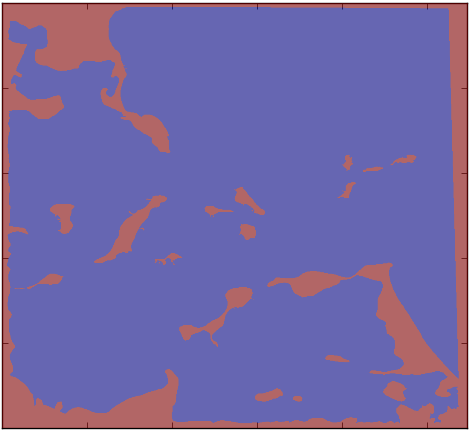
\includegraphics[width=\textwidth]{Fig_blankMap.png}
        \caption[]{{\small Environment with terrain: \\ Massachusetts Bay and surrounding area. }}    
        \label{fig:env_terrain}
    \end{subfigure}
    \hfill
    \begin{subfigure}[b]{0.475\textwidth}  
        \centering 
        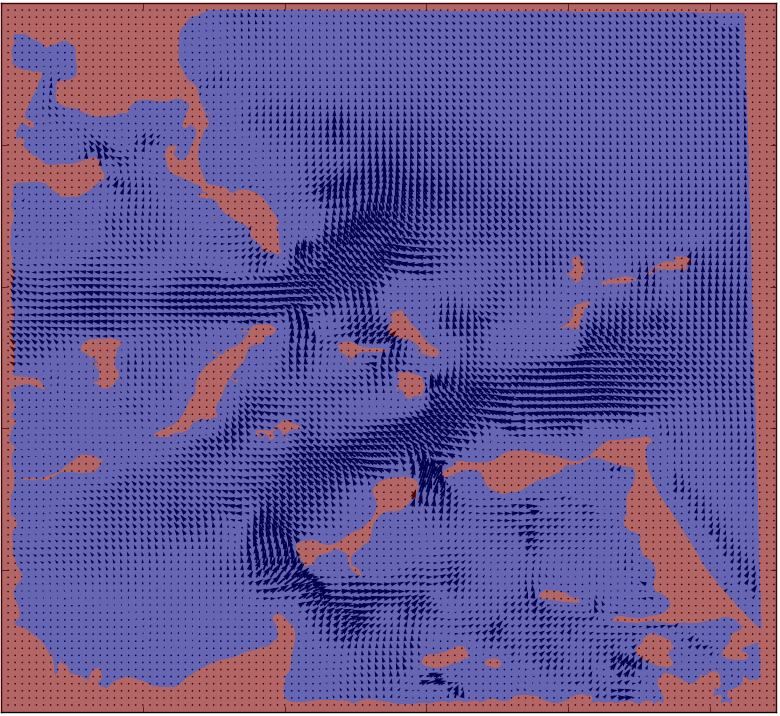
\includegraphics[width=\textwidth]{Fig_currentsMap.png}
        \caption{{\small Environment with water currents, \\ obtained from NECOFS forecast.}}   
        \label{fig:env_currents}
    \end{subfigure}
    \vskip\baselineskip
    \begin{subfigure}[b]{0.475\textwidth}   
        \centering 
        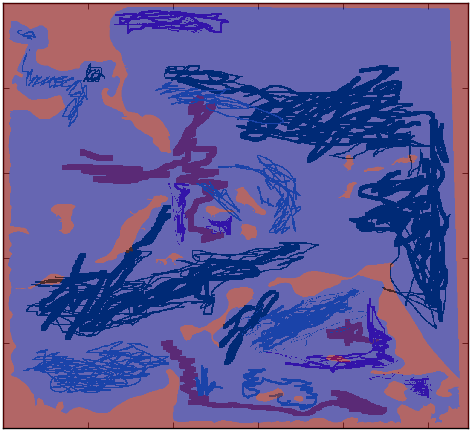
\includegraphics[width=\textwidth]{Fig_entitiesMap.png}
        \caption[]{{\small Environment with (simulated) \\ subsurface entities under study by USV.}}
        \label{fig:env_entities}
    \end{subfigure}
    \quad
    \begin{subfigure}[b]{0.475\textwidth}   
        \centering 
        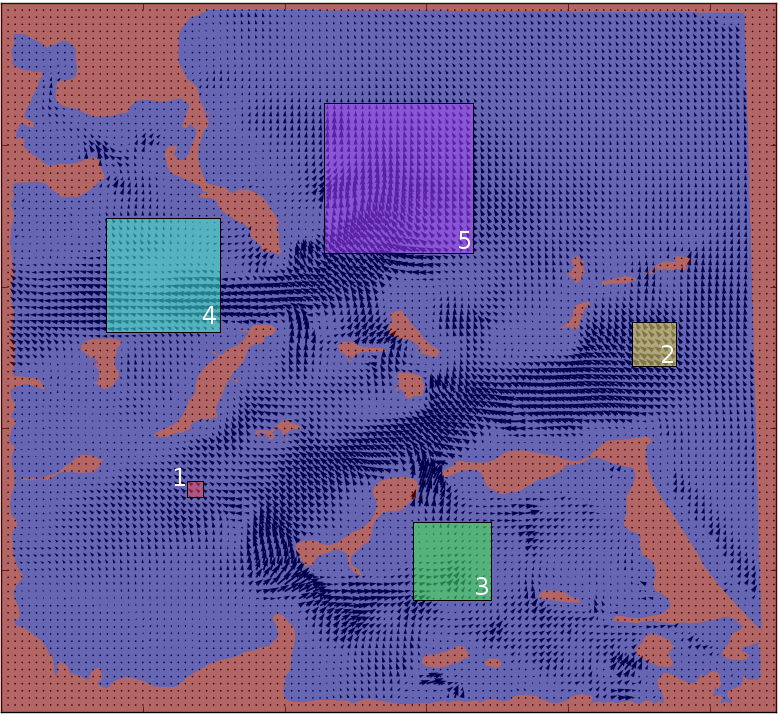
\includegraphics[width=\textwidth]{CurrentsTargetMap.png}
        \caption[]{{\small Environment with example target \\ regions $R_1, R_2, .., R_5$}}   
        \label{fig:env_targets}
    \end{subfigure}
    \caption[]{\small Environment Overview } 
    \label{fig:env}
\end{figure*}
%%%%%%%%%%%%%%%%%%%%%%%%%%
% End experimental Setup %
%%%%%%%%%%%%%%%%%%%%%%%%%%

%%%%%%%%%%%%%%%%%%%%%%%%%%%%%%%%%
% Water currents time intervals %
%%%%%%%%%%%%%%%%%%%%%%%%%%%%%%%%%
\begin{figure*}
    \captionsetup{justification=centering}
    \centering
    \begin{subfigure}[b]{0.475\textwidth}
        \centering
        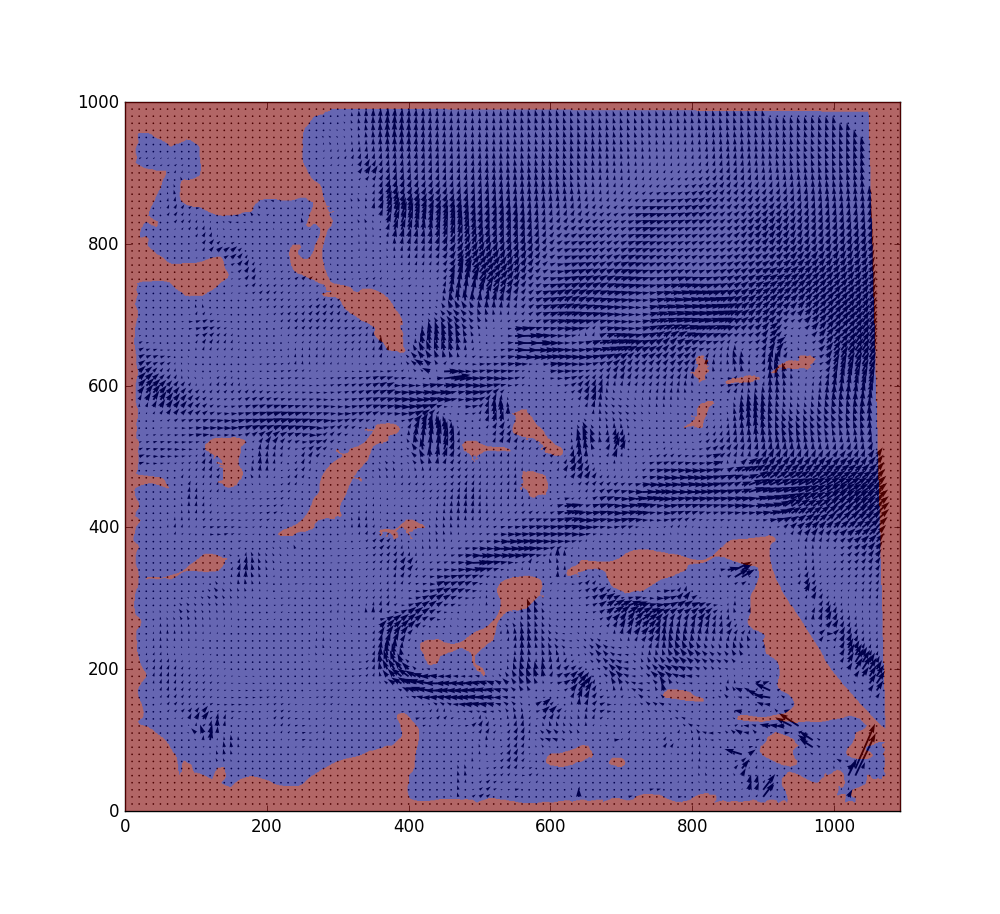
\includegraphics[width=\textwidth,trim={3cm 3cm 3cm 3cm},clip]{Fig_currentsMap-1.png}
        \caption[]{{\small Water currents at $t = 0 (min)$, $t_{interval} = 1$}}    
        \label{fig:currents_interval_1}
    \end{subfigure}
    \hfill
    \begin{subfigure}[b]{0.475\textwidth}  
        \centering 
        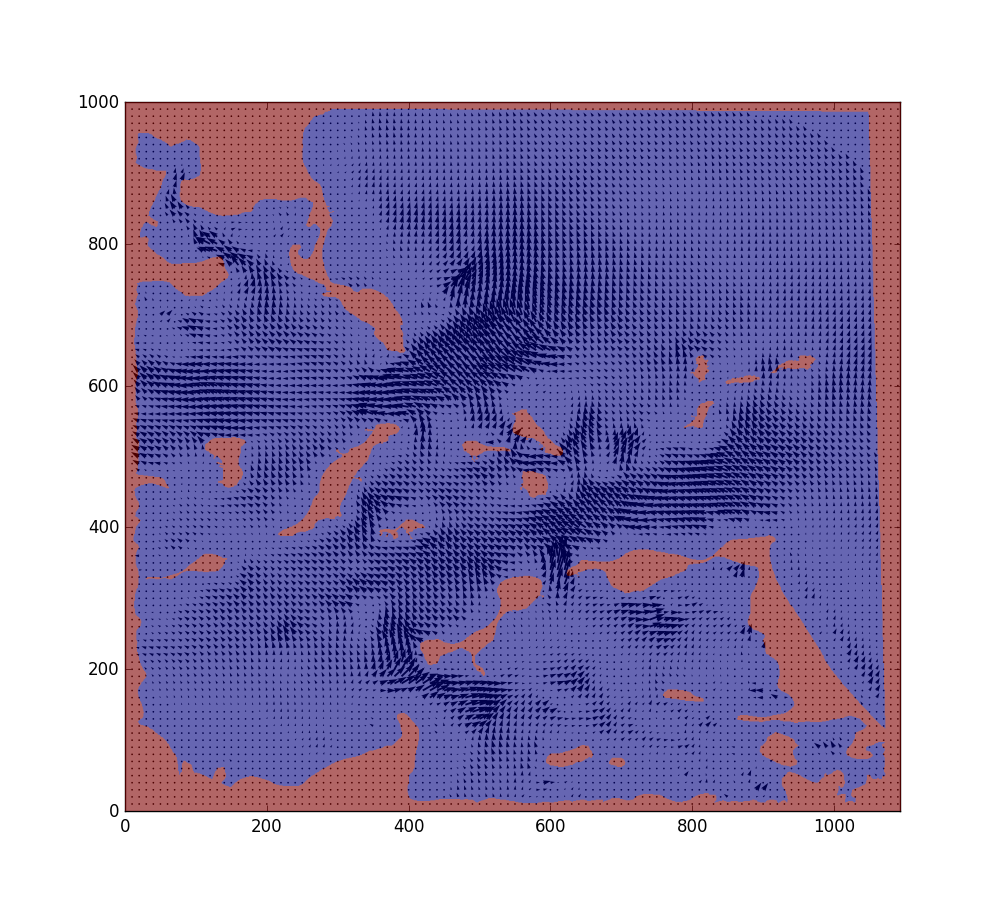
\includegraphics[width=\textwidth,trim={3cm 3cm 3cm 3cm},clip]{Fig_currentsMap-3.png}
        \caption[]{{\small Water currents at $t = 60 (min)$, $t_{interval} = 3$}}   
        \label{fig:currents_interval_3}
    \end{subfigure}
    \vskip\baselineskip
    \begin{subfigure}[b]{0.475\textwidth}   
        \centering 
        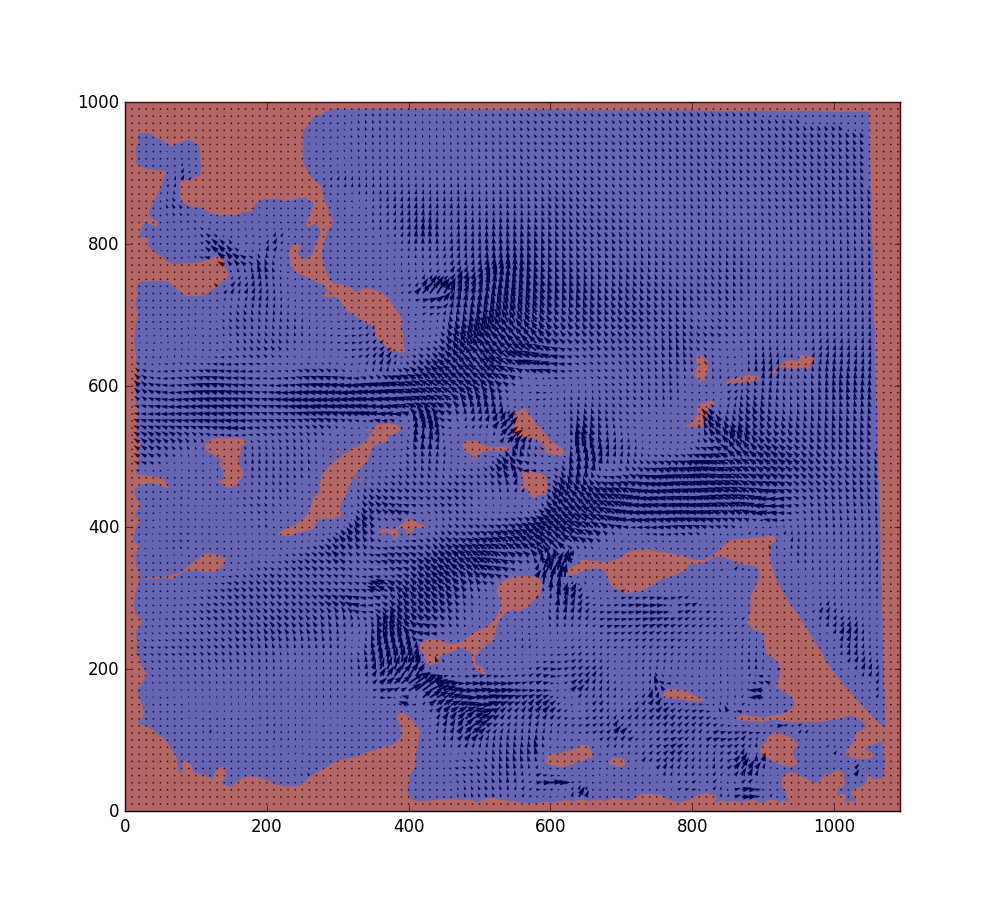
\includegraphics[width=\textwidth,trim={3cm 3cm 3cm 3cm},clip]{Fig_currentsMap-5.png}
        \caption[]{{\small Water currents at $t = 120 (min)$, $t_{interval} = 5$}}   
        \label{fig:currents_interval_5}
    \end{subfigure}
    \quad
    \begin{subfigure}[b]{0.475\textwidth}   
        \centering 
        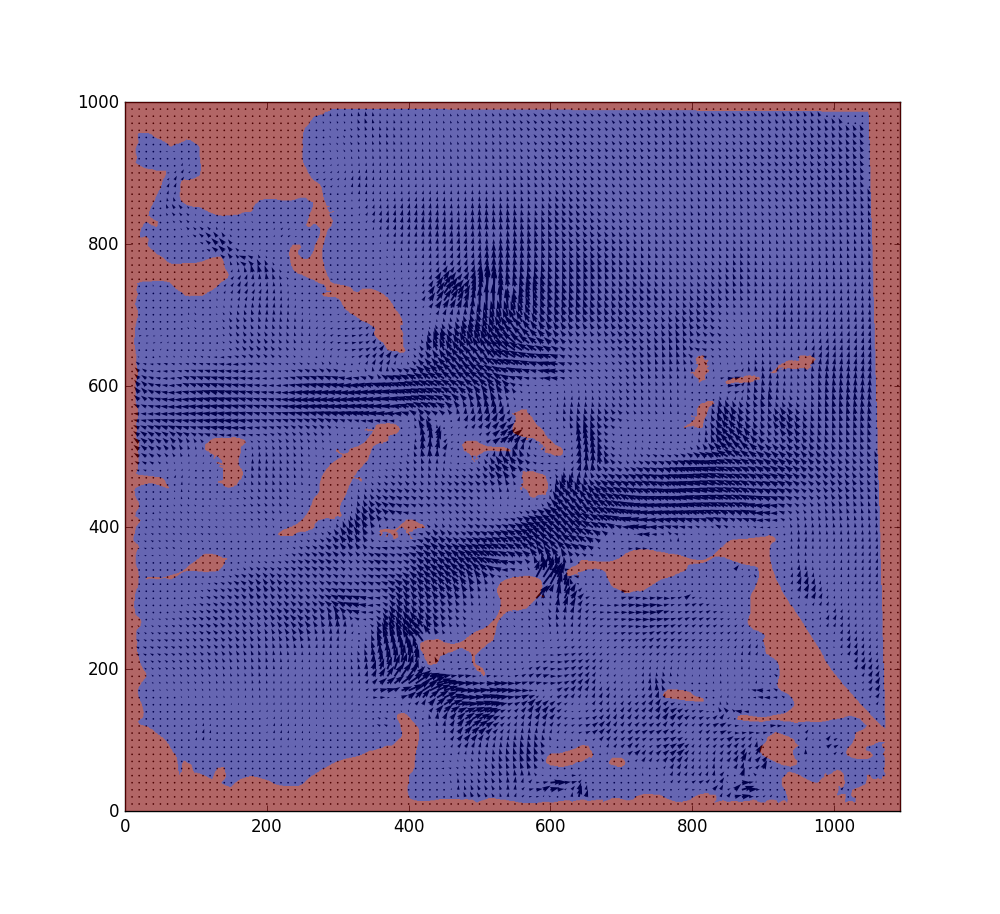
\includegraphics[width=\textwidth,trim={3cm 3cm 3cm 3cm},clip]{Fig_currentsMap-7.png}
        \caption[interval 7]%
        {{\small Water currents at $t = 180 (min)$, $t_{interval} = 7$}}   
        \label{fig:currents_interval_7}
    \end{subfigure}
    \caption[]{\small Water currents vary over time $t$ and are stored in discrete intervals $t_{interval}$.} 
    \label{fig:currents_intervals}
\end{figure*}
%%%%%%%%%%%%%%%%%%%%%%%%%%%%%%%%%%%%%
% End Water currents time intervals %
%%%%%%%%%%%%%%%%%%%%%%%%%%%%%%%%%%%%%

%%%%%%%%%%%%%%%%%
% System params %
%%%%%%%%%%%%%%%%%
\begin{table}[H]\small
    \begin{tabular}{|l|l|l|}
    \hline
    USV speed (knots) & Water current update interval (minutes) & Water current forecast duration (hours) \\
    \hline
    5                 & 30                                      & 24 \\
    \hline
    \end{tabular}
    \caption{System settings}
    \label{sys_settings}
\end{table}


\begin{table}[H]\small
    \begin{tabular}{|l|l|l|l|l|l|l|l|l|l|}
\hline
ID & Score & Lon & Lat & Width & Length & Xpoints & Ypoints & Margin & Roam \\
\hline
1 & 100 & -70.970 & 42.300 & 10 & 10 & 10 & 10 & 1 & 0 \\
\hline
2 & 100 & -70.881 & 42.327 & 50 & 50 & 50 & 50 & 1 & 0 \\
\hline
3 & 100 & -70.920 & 42.287 & 100 & 100 & 100 & 100 & 1 & 0 \\
\hline
4 & 100 & -70.976 & 42.340 & 150 & 150 & 150 & 150 & 1 & 0 \\
\hline
5 & 100 & -70.930 & 42.348 & 200 & 200 & 200 & 200 & 1 & 0 \\
\hline  
        
    \end{tabular}
    \caption{Targets for mission planning}
    \label{tbl:targets}
\end{table}

\begin{table}[H]\small
    \begin{tabular}{|l|l|l|}
\hline
ID & Lon & Lat\\
\hline
1 & -70.9869 & 42.3035 \\
\hline  
    \end{tabular}
    \caption{Safepoints. Robot must end mission at exactly one of the locations.}
    \label{tbl:safepoints}
\end{table}

\section{Surveyor Results}

\subsection{Mission Planning}

Two experiments were run to compare the missions planned by MPFC and MPTR. In the first, the maximum duration and work constraints, $D_{max}$ and $W_{max}$, are set high enough that all targets are able to visited in a feasible mission. In the second, these constraints are tightened so that MPFC and MPTR have to generate missions that optimize reward without visiting every target. The constraints for both setups are in Table \ref{tbl:constraints}.

\begin{table}[H]\small
    \begin{tabular}{|l|l|l|}
\hline
Situation & $D_{max} (minutes)$ & $W_{max} (Joules)$ \\
\hline
Visiting each target is feasible & 1000 & 10000000000 \\
\hline  
Visiting each target is infeasible &    & \\
\hline
    \end{tabular}
    \caption{Constraints used in mission planning experiments}
    \label{tbl:constraints}
\end{table}

\textbf{Section is a work in progress since I need to finish MPTR implementation}

Top 5 mission plans
[0, 5, 4, 3, 2, 1, 6]
[0, 4, 5, 3, 1, 2, 6]
[0, 3, 5, 2, 1, 4, 6]
[0, 3, 4, 5, 1, 2, 6]
[0, 3, 4, 1, 5, 2, 6]


\subsection{\textit{Goto} Path Planning}

The \textit{Goto} planning results form the bulk of the analysis, and will be used to answer some of the questions posed in Section \ref{section:contributions}. A number of runs are analyzed with variation on the weights, but all are evaluated using six \testit{Goto} tasks. Three pairs of points are selected and each yields two tasks based on reversing the start and stop points. This reversal is to ensure that the water current impacts the system enough that the direction of planning affects the result over them same area. The six paths are described in Table \ref{tbl:goto_tasks}.

\begin{table}[H]\small
    \begin{tabular}{|l|l|l|l|l|l|l|l|l|l|l|l|}
    \hline
    \thead{Goto task} & \thead{Source \\ (node)}  & \thead{Source \\ (Lat)} & \thead{Source \\ (Lon)} 
                 &  \thead{Goal \\ (node)}  & \thead{Goal \\ (Lat)} & \thead{Goal \\ (Lon)}\\
    \hline
    1-A & 1 & 42.300 & -70.970 & 5 &  42.348 & -70.930 \\
    \hline
    1-B & 5 & 42.348 & -70.930 & 1 &  42.300 & -70.970 \\
    \hline
    2-A & 5 & 42.348 & -70.930 & 2 & -70.881 &  42.327 \\
    \hline
    2-B & 2 & -70.881 & 42.327 & 5 &  42.348 & -70.930 \\
    \hline
    3-A & 1 & 42.300 & -70.970 & 3 & -70.920 &  42.287 \\
    \hline
    3-B & 3 & -70.920 &  42.287 & 1 & 42.300 & -70.970  \\
    \hline
    \end{tabular}
    \caption{\textit{Goto} tasks for path planning experiments. Node labels correspond to the target IDs in \ref{fig:env_targets}, and the coordinates are the region's center}
    \label{tbl:goto_tasks}
\end{table}

\subsubsection{Initial Visual Analysis}
\ref{section:initial_results}
\textit{Goto} analysis begins with a visual check that the paths are reasonable and that the various optimization criteria affect paths in the way that would be expected. The initial weights were selected by trial and error during development of the fitness function. No attempt has been made to refine the weights to achieve a desired behavior other than checking that the obstacles are avoided and that the paths make reasonably efficient waypoint placement. The work and reward criteria are toggled off and on to see how they affect the path separately and together. The solution paths for this experiment are shown in Figures \ref{fig:Paths_1-A_1-B}, \ref{fig:Paths_1-A_1-B}, and \ref{fig:Paths_1-A_1-B}. Each figure contains subfigures where the left-hand subfigures are runs for the 'A' \textit{Goto} tasks and the right-hand are for 'B' between the same two points. In all cases, the obstacle avoidance and distance minimization criteria are enabled.

When work and reward are both disabled, the behavior is as expected. When a straight line exists between the points (Figure \ref{}, \ref{}), the waypoint align along that line. In the presence of obstacles, the waypoints are positioned to tightly approach the shoreline to avoid collision with minimal deviation. Since the work criteria is disabled, there is no difference in the problem when reversing the start and end points of a path. This is demonstrated by the low variability between 'A' and 'B' paths under terrain and distance-only optimization. When adding only work minimization, the paths exhibit some variation. In \textit{Task 1-A}, the currents support the mission and no visible change is made to the path. From the other direction, \textit{Task 1-B}, a path deviation is made to avoid currents that require additional energy consumption. Comparing \textit{Task 2-A} and \textit{Task 2-B}, the currents influence the decision of which direction to go when routing around an island obstacle. Subtle changes are similarly present in \textit{Task 3-A} and \textit{Task 3-B}. It should be acknowledged that some deviation is almost assured when using metaheuristic solvers, but it will be shown that the convergence is tight. That all scenarios showed stronger deviation with work considered than without suggests that the work optimization is behaving as expected. In all cases, the result when only reward is added shows huge deviation. These paths are clearly much longer than previously planned. When reward and work are incorporated, the reward maximization dominates the work minimization. Figures \ref{fig:Path_3-A_terrain_work_reward} and \ref{fig:Path_2-A_terrain_work_reward} do show some bounding of the path toward the solution without reward criteria. The first major observation of these experiments is that every path is affected by the additional criteria in ways that match expectation. Second, combined criteria exhibit characteristics of all criteria, but will require balancing to achieve the desired planning behavior.

\subsubsection{Comparison of Metaheuristic Planning Algorithms}

The four metaheuristic algorithms discussed in Section \label{section:goto} are applied to path planning used the fitness function in Section \ref{section:fitness_function}. The initial results in Section \ref{section:initial_results} used PSO, which was arbitrarily chosen. A suitable algorithm repeatedly reaches an approximately optimal solution within a bounded number of iterations. 


%%%%%%%%%%%%%%%%%%%%%%%%%%%%%%%%%
% Convergence curves %
%%%%%%%%%%%%%%%%%%%%%%%%%%%%%%%%%
\begin{figure*}
    \captionsetup{justification=centering}
    \centering
        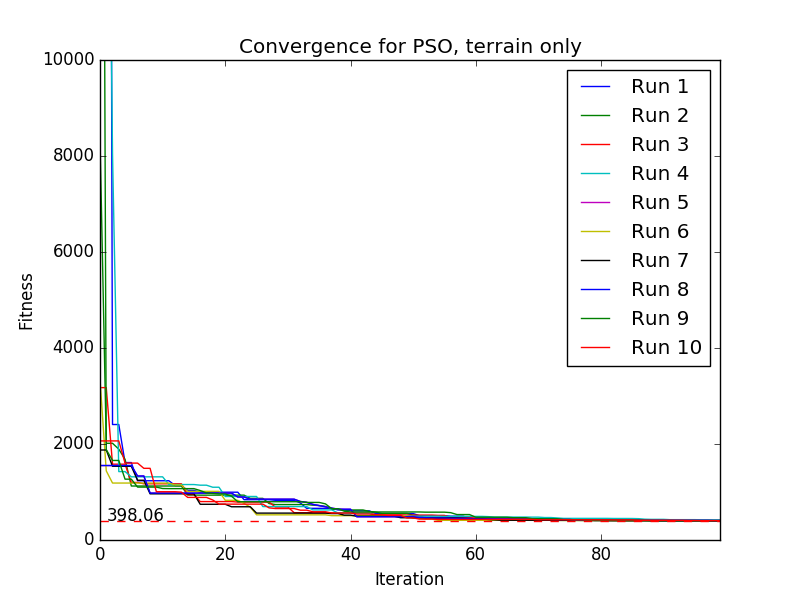
\includegraphics[width=0.75\textwidth]{conv_PSO_a.png}
    \caption[]{{\small Convergence for particle swarm optimization}}
    \label{fig:convergence_a_PSO}
\end{figure*}

\begin{figure*}
    \captionsetup{justification=centering}
    \centering
        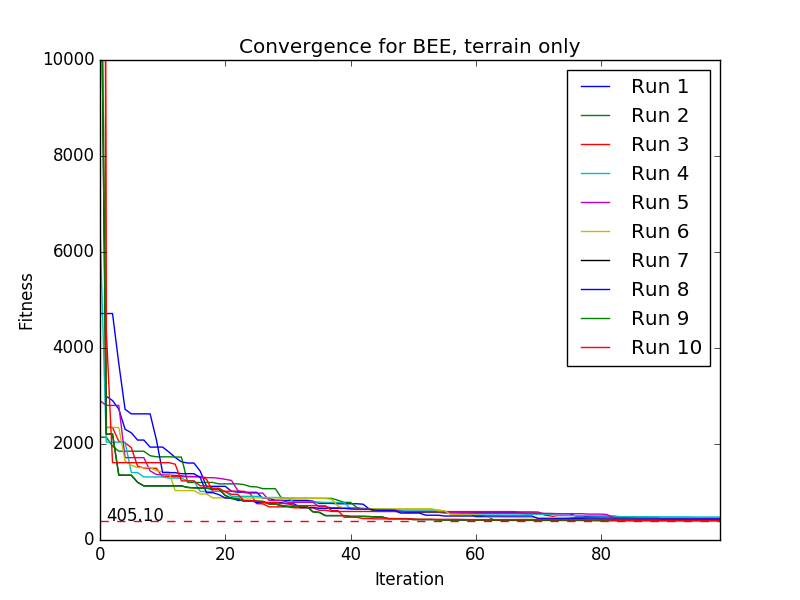
\includegraphics[width=0.75\textwidth]{conv_BEE_a.png}
    \caption[]{{\small Convergence for bee colony optimization }}
    \label{fig:convergence_a_BEE}
\end{figure*}

\begin{figure*}
    \captionsetup{justification=centering}
    \centering
        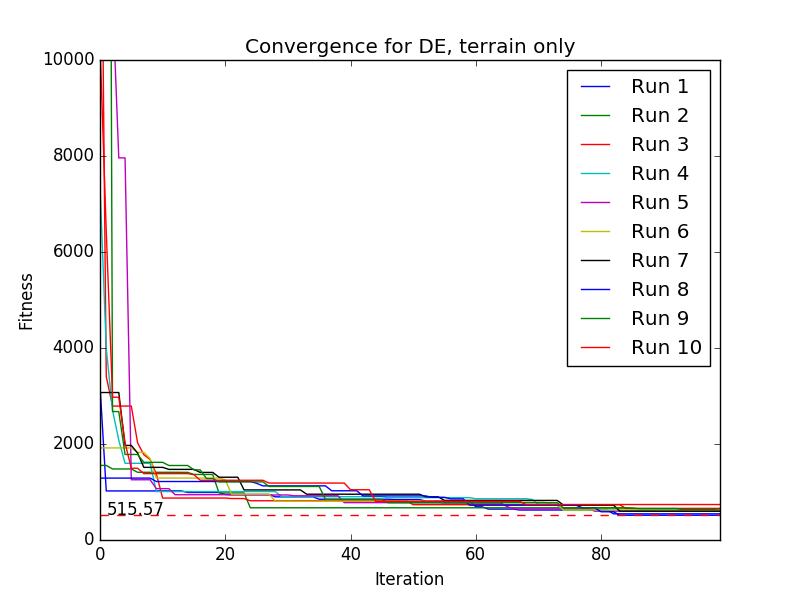
\includegraphics[width=0.75\textwidth]{conv_DE_a.png}
    \caption[]{{\small Convergence for differential evolution}}   
    \label{fig:convergence_a_DE}
\end{figure*}

\begin{figure*}
    \captionsetup{justification=centering}
    \centering
        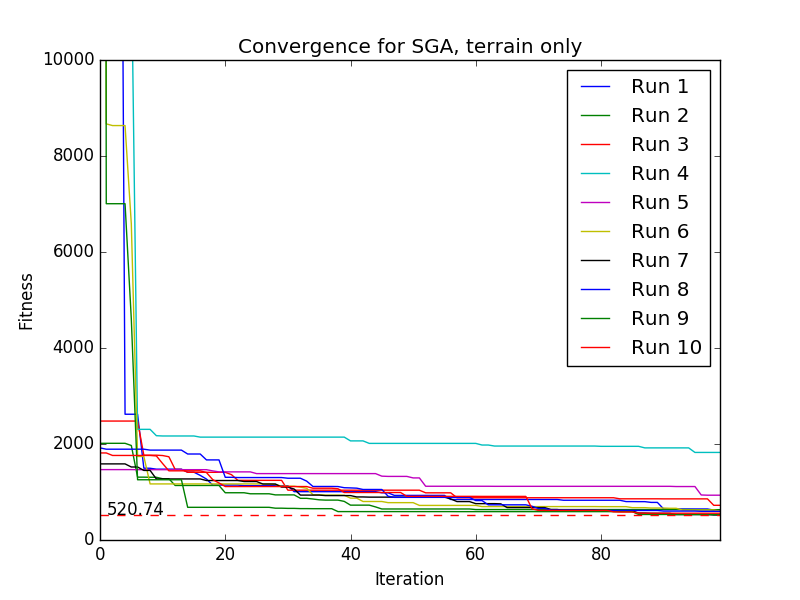
\includegraphics[width=0.75\textwidth]{conv_SGA_a.png}
    \caption[]{{\small Convergence for genetic algorithm}}   
    \label{fig:convergence_a_SGA}
\end{figure*}



\begin{figure*}
    \captionsetup{justification=centering}
    \centering
    \begin{subfigure}[b]{0.475\textwidth}
        \centering
        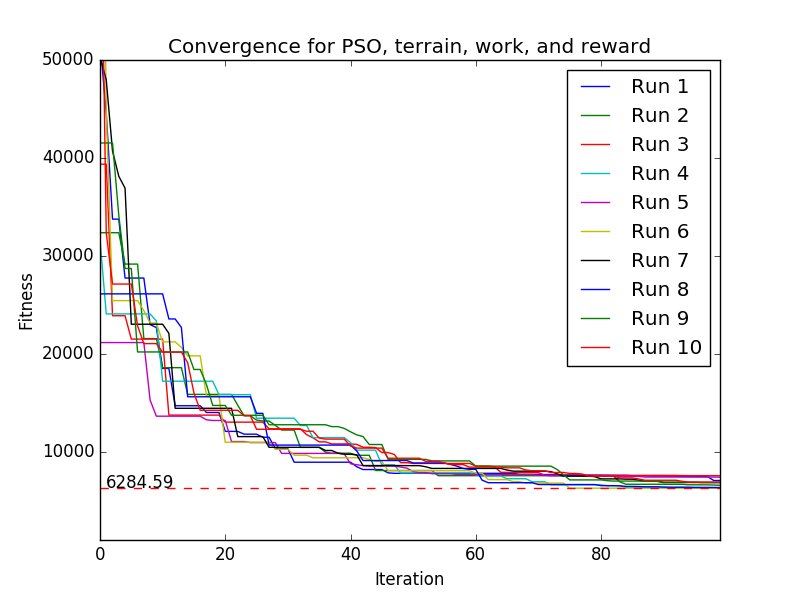
\includegraphics[width=\textwidth]{conv_PSO_b.png}
        \caption[]{{\small Convergence for particle swarm optimization}}
        \label{fig:convergence_b_PSO}
    \end{subfigure}
    \hfill
    \begin{subfigure}[b]{0.475\textwidth}  
        \centering 
        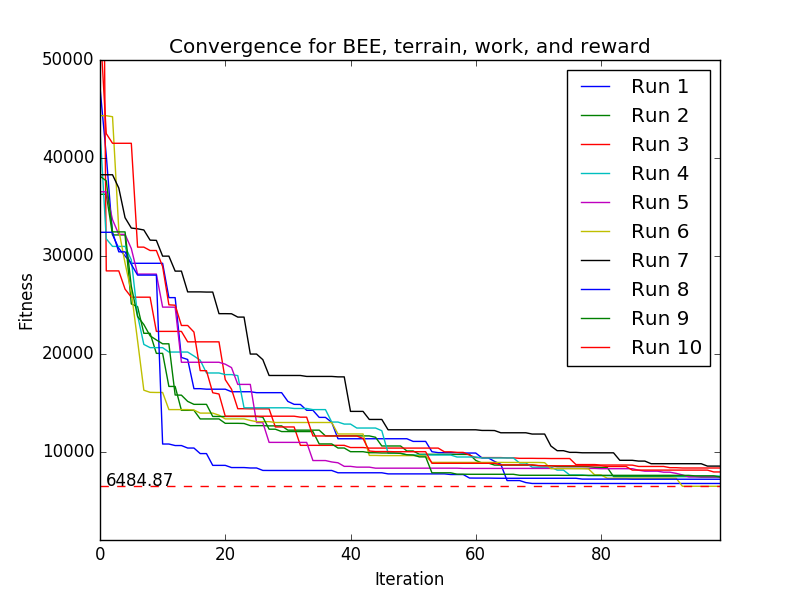
\includegraphics[width=\textwidth]{conv_BEE_b.png}
        \caption[]{{\small Convergence for bee colony optimization }}
        \label{fig:convergence_b_BEE}
    \end{subfigure}
    \vskip\baselineskip
    \begin{subfigure}[b]{0.475\textwidth}   
        \centering 
        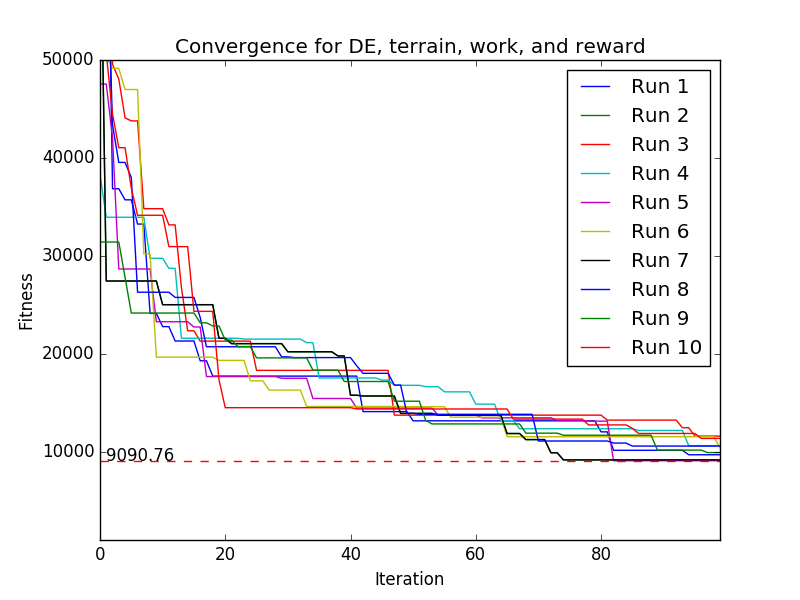
\includegraphics[width=\textwidth]{conv_DE_b.png}
        \caption[]{{\small Convergence for differential evolution}}   
        \label{fig:convergence_b_DE}
    \end{subfigure}
    \quad
    \begin{subfigure}[b]{0.475\textwidth}   
        \centering 
        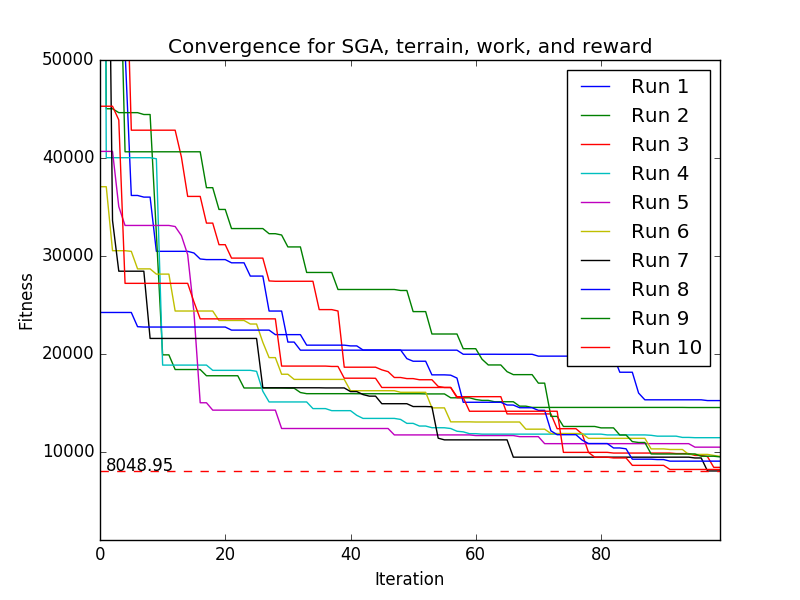
\includegraphics[width=\textwidth]{conv_SGA_b.png}
        \caption[]{{\small Convergence for genetic algorithm}}   
        \label{fig:convergence_b_SGA}
    \end{subfigure}
    \caption[]{\small Convergence curves for four metaheuristic algorithms applied to path planning \\ (considering terrain, distance, work, reward)} 
    \label{fig:convergence_b}
\end{figure*}
%%%%%%%%%%%%%%%%%%%%%%%%%%
% End convergence curves %
%%%%%%%%%%%%%%%%%%%%%%%%%%


%%%%%%%%%%%%%%%%%%%%%
% Algorithm compare %
%%%%%%%%%%%%%%%%%%%%%
\begin{figure*}
    \captionsetup{justification=centering}
    \centering
    \begin{subfigure}[b]{0.475\textwidth}
        \centering
        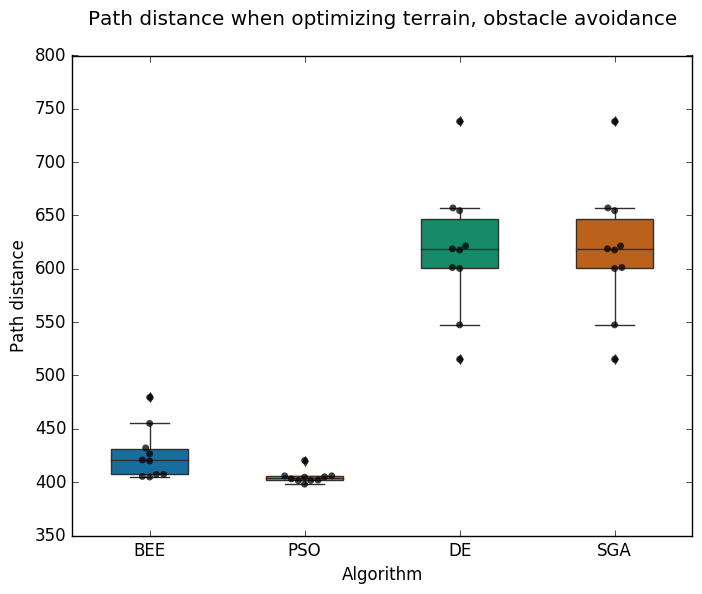
\includegraphics[width=\textwidth]{EXP3_histo_distance_a.png}
        \caption[]{{\small Convergence for particle swarm optimization}}
        \label{fig:algcompare_a_distance}
    \end{subfigure}
    \hfill
    \begin{subfigure}[b]{0.475\textwidth}  
        \centering 
        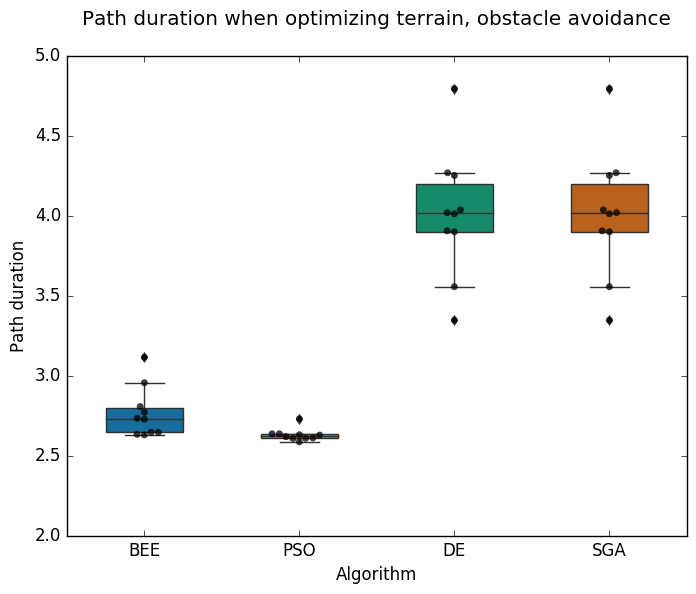
\includegraphics[width=\textwidth]{EXP3_histo_duration_a.png}
        \caption[]{{\small Convergence for bee colony optimization }}
        \label{fig:algcompare_a_duration}
    \end{subfigure}
    \vskip\baselineskip
    \begin{subfigure}[b]{0.475\textwidth}   
        \centering 
        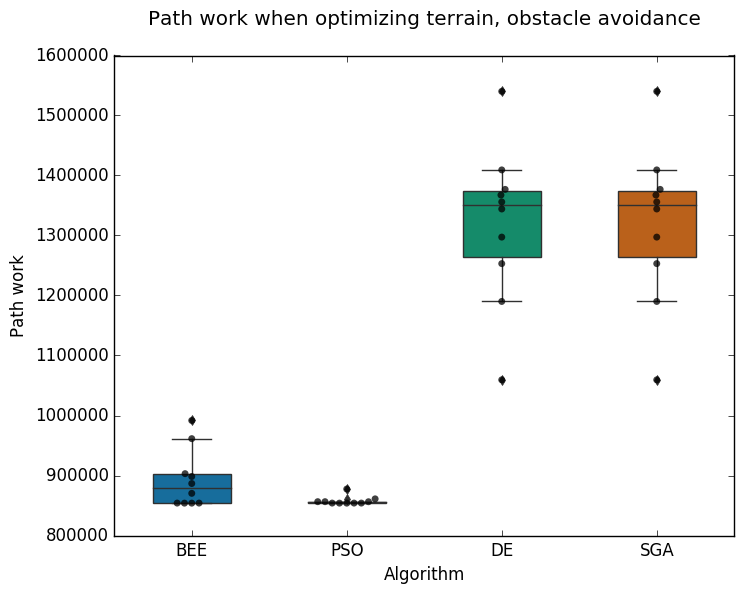
\includegraphics[width=\textwidth]{EXP3_histo_work_a.png}
        \caption[]{{\small Convergence for differential evolution}}   
        \label{fig:algcompare_a_work}
    \end{subfigure}
    \quad
    \begin{subfigure}[b]{0.475\textwidth}   
        \centering 
        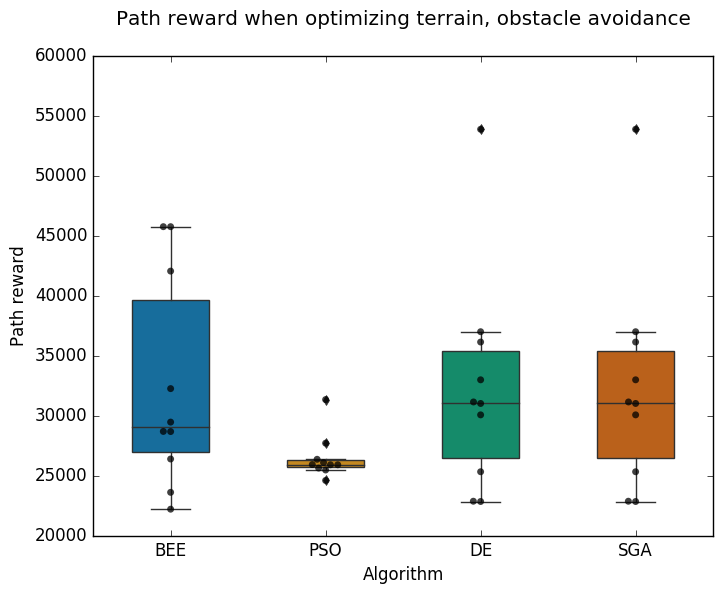
\includegraphics[width=\textwidth]{EXP3_histo_reward_a.png}
        \caption[]{{\small Convergence for genetic algorithm}}   
        \label{fig:algcompare_a_reward}
    \end{subfigure}
    \caption[]{\small Convergence curves for four metaheuristic algorithms applied to path planning \\ (considering terrain and distance)} 
    \label{fig:algcompare_a}
\end{figure*}

\begin{figure*}
    \captionsetup{justification=centering}
    \centering
    \begin{subfigure}[b]{0.475\textwidth}
        \centering
        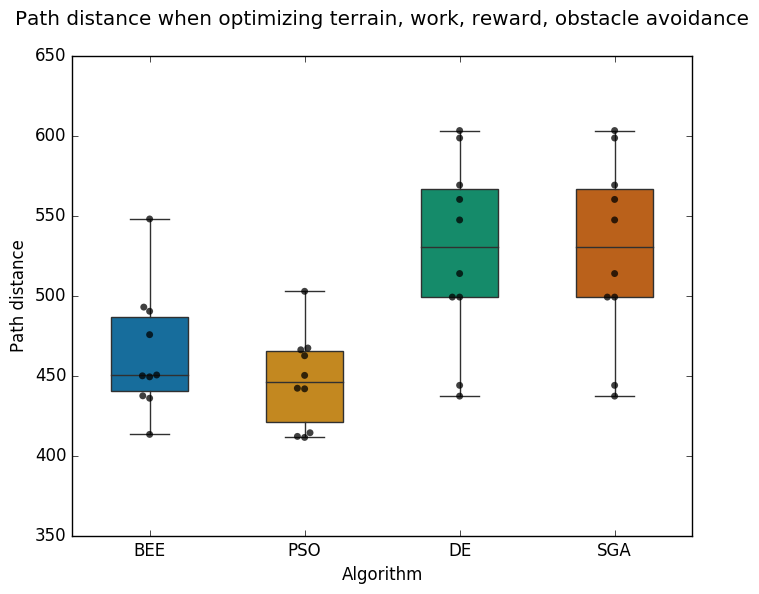
\includegraphics[width=\textwidth]{EXP3_histo_distance_b.png}
        \caption[]{{\small Convergence for particle swarm optimization}}
        \label{fig:algcompare_b_distance}
    \end{subfigure}
    \hfill
    \begin{subfigure}[b]{0.475\textwidth}  
        \centering 
        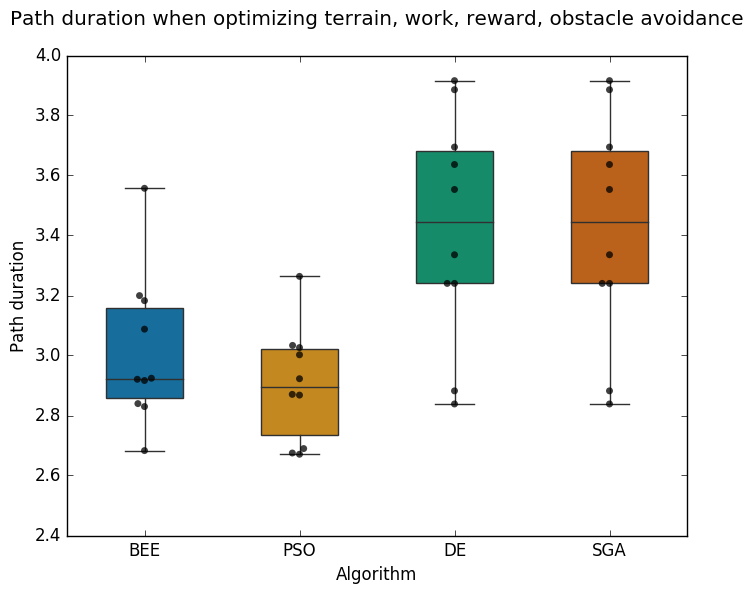
\includegraphics[width=\textwidth]{EXP3_histo_duration_b.png}
        \caption[]{{\small Convergence for bee colony optimization }}
        \label{fig:algcompare_b_duration}
    \end{subfigure}
    \vskip\baselineskip
    \begin{subfigure}[b]{0.475\textwidth}   
        \centering 
        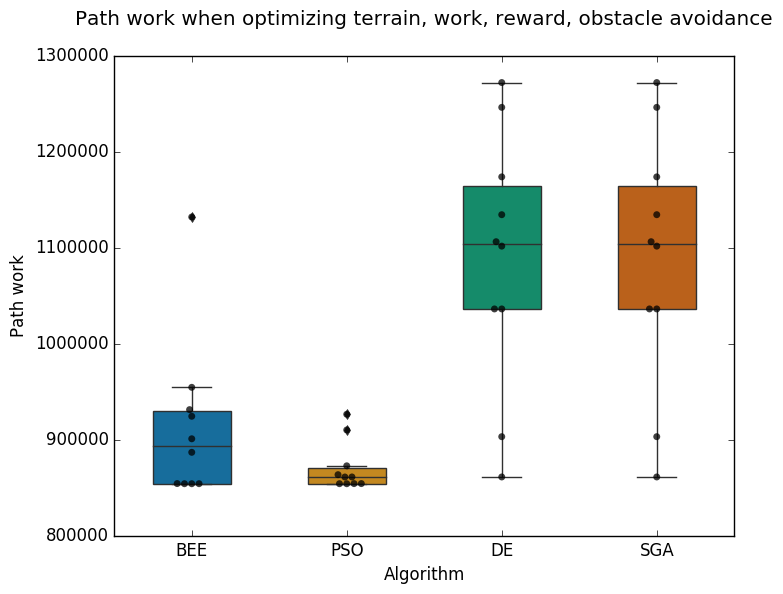
\includegraphics[width=\textwidth]{EXP3_histo_work_b.png}
        \caption[]{{\small Convergence for differential evolution}}   
        \label{fig:algcompare_b_work}
    \end{subfigure}
    \quad
    \begin{subfigure}[b]{0.475\textwidth}   
        \centering 
        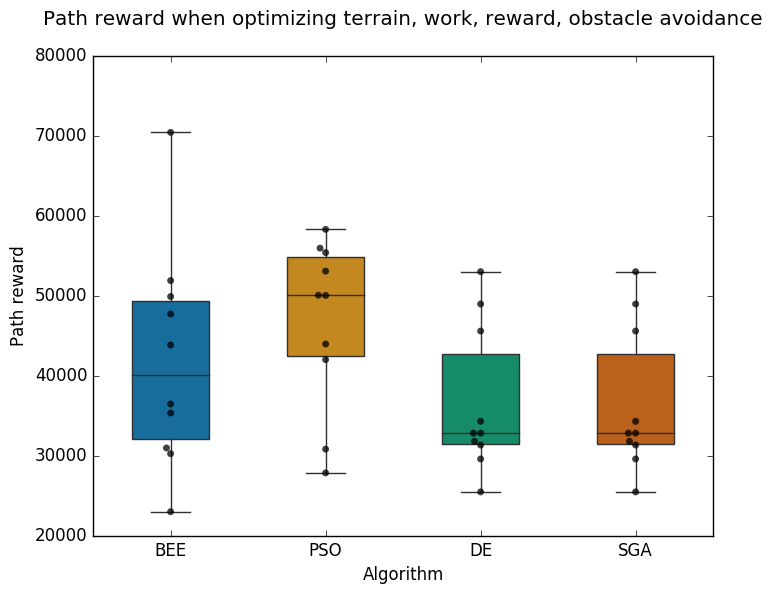
\includegraphics[width=\textwidth]{EXP3_histo_reward_b.png}
        \caption[]{{\small Convergence for genetic algorithm}}   
        \label{fig:algcompare_b_reward}
    \end{subfigure}
    \caption[]{\small Convergence curves for four metaheuristic algorithms applied to path planning \\ (considering terrain, distance, work, reward)} 
    \label{fig:algcompare_b}
\end{figure*}
%%%%%%%%%%%%%%%%%%%%%%%%%
% End algorithm compare %
%%%%%%%%%%%%%%%%%%%%%%%%%








%%%%%%%%%%%%%%%%%%%%%%%%%%%%%
% Goto planner PSO Settings %
%%%%%%%%%%%%%%%%%%%%%%%%%%%%%
\begin{table}[H]
    \begin{tabular}{|l|l|l|}
        \hline
        \thead{Generations} & \thead{Individuals \\ (Pool size)}  & \thead{Number of waypoints}  \\
        \hline
        100 & 100 & 5   \\
        \hline
    \end{tabular}
    \caption{Settings common to all metaheuristic algorithms used. To avoid overfitting to the experimental setup, the algorithm-specific settings are unchanged from the PyGMO library defaults.}
    \label{tbl:meta_params}
\end{table}

%%%%%%%%%%%%%%%%%%%%%%%%%%%
% Goto paths for 1-A, 1-B %
%%%%%%%%%%%%%%%%%%%%%%%%%%%
\begin{figure*}
    \centering
    \begin{subfigure}[b]{0.4\textwidth}
        \centering
        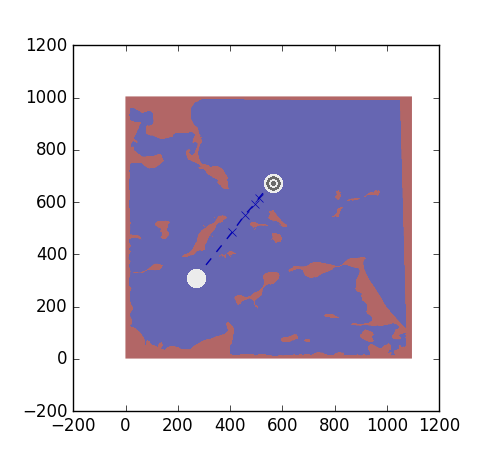
\includegraphics[width=\textwidth,trim={3cm 3cm 3cm 3cm},clip]{EXP3RG_PathAa_-1_-1_0_0.png}
        \caption[]{{\small Task 1-A, terrain only}}
        \label{fig:Path_1-A_terrain_only}
    \end{subfigure}
    \hfill
    \begin{subfigure}[b]{0.4\textwidth}  
        \centering 
        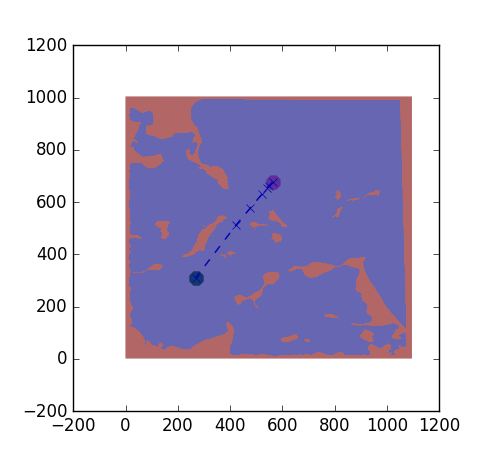
\includegraphics[width=\textwidth,trim={3cm 3cm 3cm 3cm},clip]{EXP3RG_PathAb_-1_-1_0_0.png}
        \caption[]{{\small Task 1-B, terrain only}}   
        \label{fig:Path_1-B_terrain_only}
    \end{subfigure}
    
    \begin{subfigure}[b]{0.4\textwidth}
        \centering
        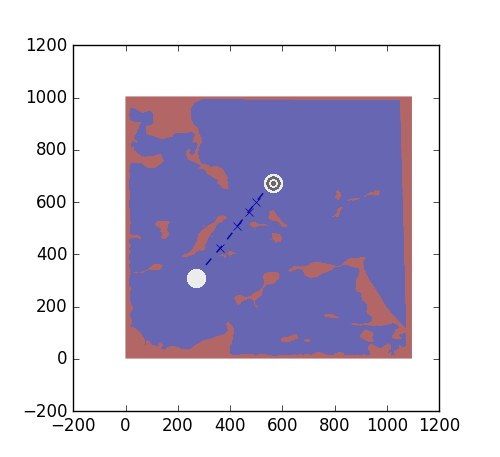
\includegraphics[width=\textwidth,trim={3cm 3cm 3cm 3cm},clip]{EXP3RG_PathAa_-1_-1_-1_0.png}
        \caption[]{{\small Task 1-A, terrain + work}}    
        \label{fig:Path_1-A_terrain_work}
    \end{subfigure}
    \hfill
    \begin{subfigure}[b]{0.4\textwidth}  
        \centering 
        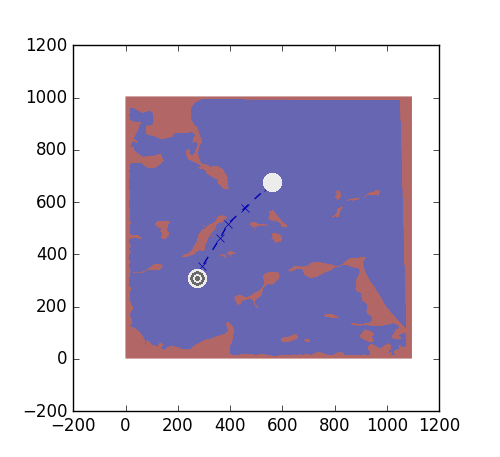
\includegraphics[width=\textwidth,trim={3cm 3cm 3cm 3cm},clip]{EXP3RG_PathAb_-1_-1_-1_0.png}
        \caption[]{{\small Task 1-B, terrain + work}}   
        \label{fig:Path_1-B_terrain_work}
    \end{subfigure}

    \begin{subfigure}[b]{0.4\textwidth}
        \centering
        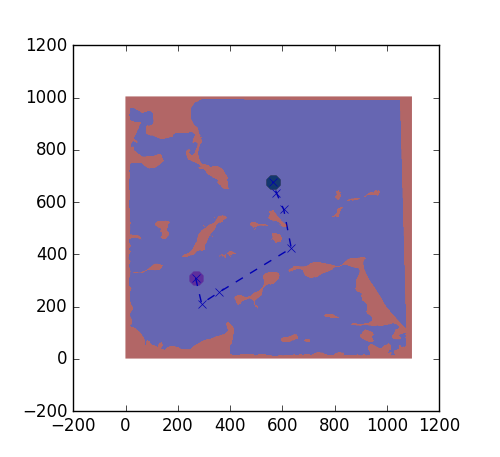
\includegraphics[width=\textwidth,trim={3cm 3cm 3cm 3cm},clip]{EXP3RG_PathAa_-1_-1_0_-1.png}
        \caption[]{{\small Task 1-A, terrain + reward}}    
        \label{fig:Path_1-A_terrain_reward}
    \end{subfigure}
    \hfill
    \begin{subfigure}[b]{0.4\textwidth}  
        \centering 
        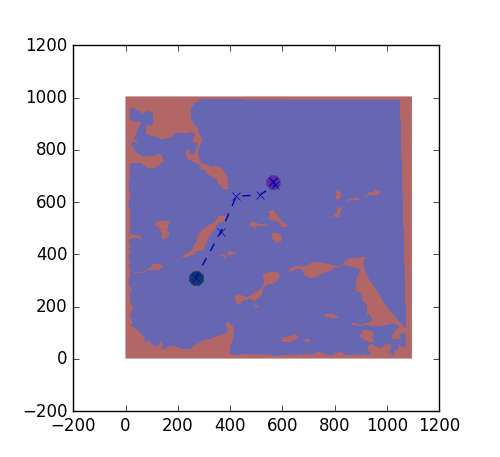
\includegraphics[width=\textwidth,trim={3cm 3cm 3cm 3cm},clip]{EXP3RG_PathAb_-1_-1_0_-1.png}
        \caption[]{{\small Task 1-B, terrain + reward}}   
        \label{fig:Path_1-B_terrain_reward}
    \end{subfigure}
   
  \begin{subfigure}[b]{0.4\textwidth}
        \centering
        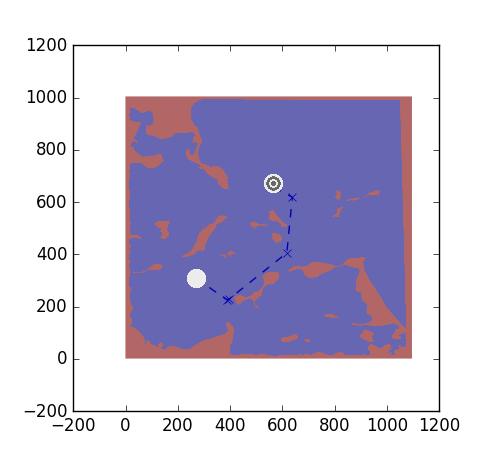
\includegraphics[width=\textwidth,trim={3cm 3cm 3cm 3cm},clip]{EXP3RG_PathAa_-1_-1_-1_-1.png}
        \caption[]{{\small Path 1-A, terrain + work + reward}}
        \label{fig:Path_1-A_terrain_work_reward}
    \end{subfigure}
    \hfill
    \begin{subfigure}[b]{0.4\textwidth}  
        \centering 
        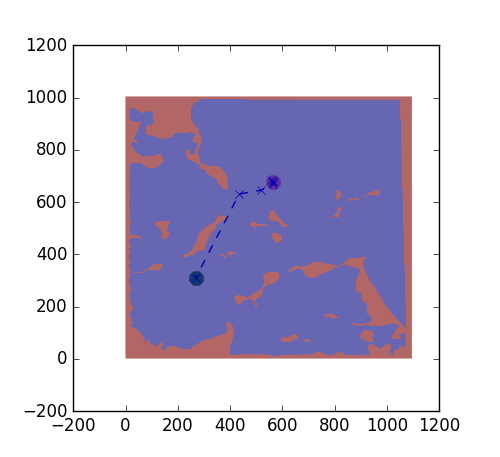
\includegraphics[width=\textwidth,trim={3cm 3cm 3cm 3cm},clip]{EXP3RG_PathAb_-1_-1_-1_-1.png}
        \caption[]{{\small Task 1-B, terrain + work + reward}}
        \label{fig:Path_5-B_terrain_work_reward}
    \end{subfigure}
      
    \caption[]{\small Solution paths for tasks 1-A and 1-B, with and without work and reward concerns.} 
    \label{fig:Paths_1-A_1-B}
\end{figure*}
%%%%%%%%%%%%%%%%%%%%%%%%%%%%%%
%End Goto paths for 1-A, 1-B %
%%%%%%%%%%%%%%%%%%%%%%%%%%%%%%

%%%%%%%%%%%%%%%%%%%%%%%%%%%
% Goto paths for 2-A, 2-B %
%%%%%%%%%%%%%%%%%%%%%%%%%%%
\begin{figure*}
    \centering
    \begin{subfigure}[b]{0.4\textwidth}
        \centering
        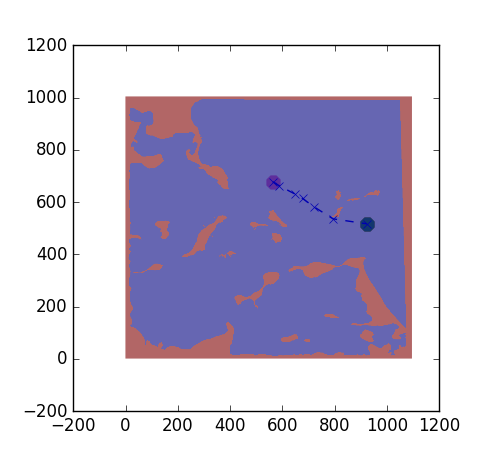
\includegraphics[width=\textwidth,trim={4cm 3cm 2cm 3cm},clip]{EXP3RG_PathBa_-1_-1_0_0.png}
        \caption[]{{\small Task 2-A, terrain only}}    
        \label{fig:Path_2-A_terrain}
    \end{subfigure}
    \hfill
    \begin{subfigure}[b]{0.4\textwidth}  
        \centering 
        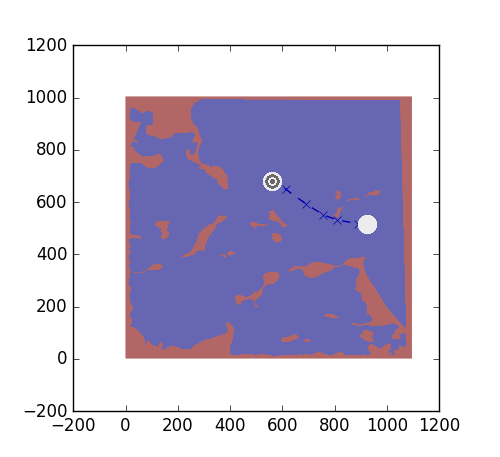
\includegraphics[width=\textwidth,trim={4cm 3cm 2cm 3cm},clip]{EXP3RG_PathBb_-1_-1_0_0.png}
        \caption[]{{\small Task 2-B, terrain only}}   
        \label{fig:Path_2-B_terrain}
    \end{subfigure}
    
    \begin{subfigure}[b]{0.4\textwidth}
        \centering
        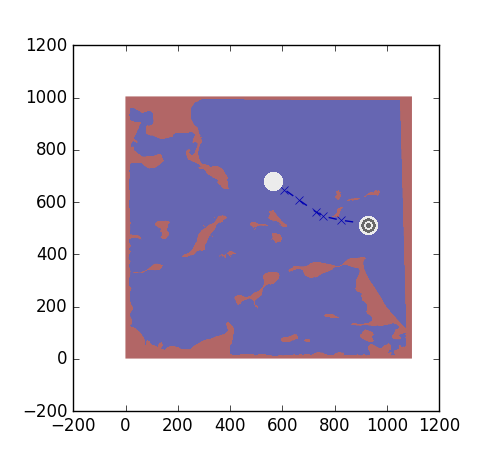
\includegraphics[width=\textwidth,trim={4cm 3cm 2cm 3cm},clip]{EXP3RG_PathBa_-1_-1_-1_0.png}
        \caption[]{{\small Task 2-A, terrain + work}}    
        \label{fig:Path_2-A_terrain_work}
    \end{subfigure}
    \hfill
    \begin{subfigure}[b]{0.4\textwidth}  
        \centering 
        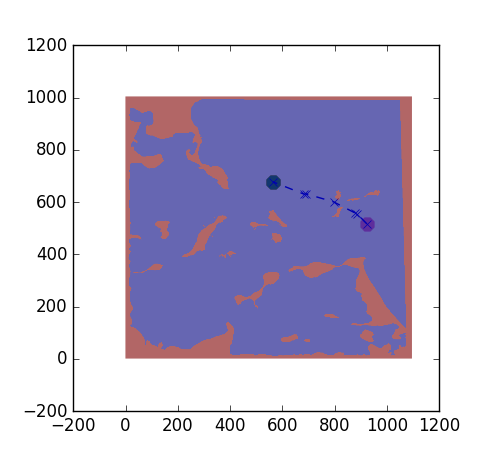
\includegraphics[width=\textwidth,trim={4cm 3cm 2cm 3cm},clip]{EXP3RG_PathBb_-1_-1_-1_0.png}
        \caption[]{{\small Task 2-B, terrain + work}}   
        \label{fig:Path_2-B_terrain_work}
    \end{subfigure}

    \begin{subfigure}[b]{0.4\textwidth}
        \centering
        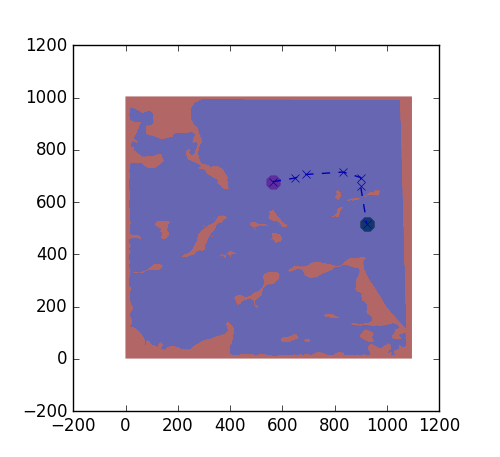
\includegraphics[width=\textwidth,trim={4cm 3cm 2cm 3cm},clip]{EXP3RG_PathBa_-1_-1_0_-1.png}
        \caption[]{{\small Task 2-A, terrain + reward}}    
        \label{fig:Path_2-A_terrain_reward}
    \end{subfigure}
    \hfill
    \begin{subfigure}[b]{0.4\textwidth}  
        \centering 
        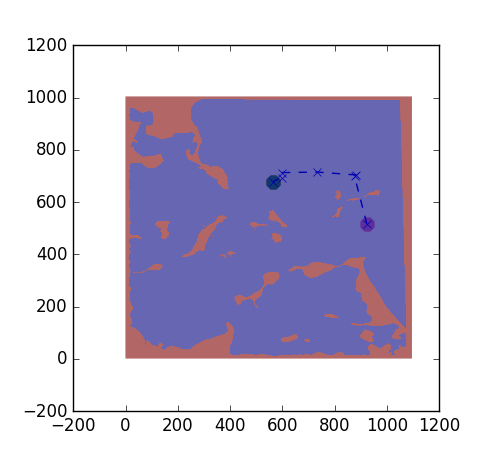
\includegraphics[width=\textwidth,trim={4cm 3cm 2cm 3cm},clip]{EXP3RG_PathBb_-1_-1_0_-1.png}
        \caption[]{{\small Task 2-B, terrain + reward}}   
        \label{fig:Path_2-B_terrain_reward}
    \end{subfigure}
    
  \begin{subfigure}[b]{0.4\textwidth}
        \centering
        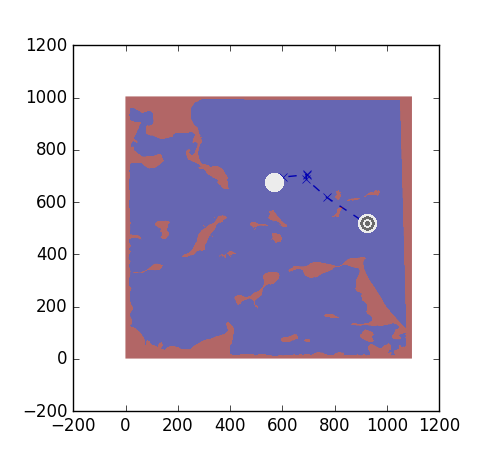
\includegraphics[width=\textwidth,trim={4cm 3cm 2cm 3cm},clip]{EXP3RG_PathBa_-1_-1_-1_-1.png}
        \caption[]{{\small Task 2-A, terrain + work + reward}}    
        \label{fig:Path_2-A_terrain_work_reward}
    \end{subfigure}
    \hfill
    \begin{subfigure}[b]{0.4\textwidth}  
        \centering 
        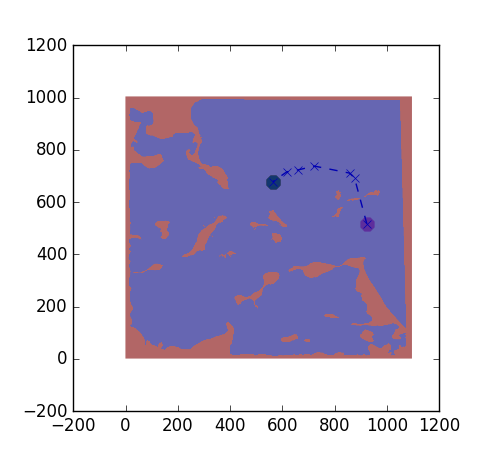
\includegraphics[width=\textwidth,trim={4cm 3cm 2cm 3cm},clip]{EXP3RG_PathBb_-1_-1_-1_-1.png}
        \caption[]{{\small Task 2-B, terrain + work + reward}}   
        \label{fig:Path_2-B_terrain_work_reward}
    \end{subfigure}

    \caption[]{\small Solution paths for tasks 2-A and 2-B, with and without work and reward concerns.} 
    \label{fig:Paths_2-A_2-B}
\end{figure*}
%%%%%%%%%%%%%%%%%%%%%%%%%%%%%%
%End Goto paths for 2-A, 2-B %
%%%%%%%%%%%%%%%%%%%%%%%%%%%%%%

%%%%%%%%%%%%%%%%%%%%%%%%%%%
% Goto paths for 3-A, 3-B %
%%%%%%%%%%%%%%%%%%%%%%%%%%%
\begin{figure*}
    \centering
    \begin{subfigure}[b]{0.4\textwidth}
        \centering
        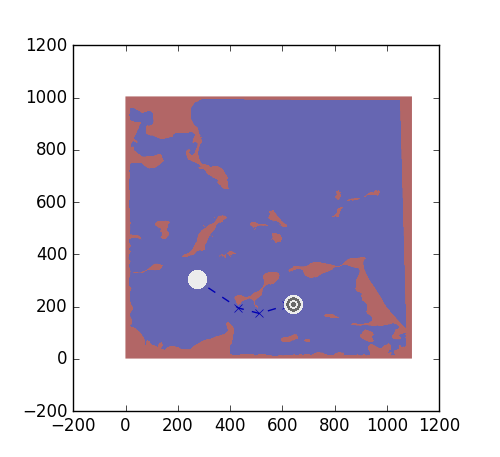
\includegraphics[width=\textwidth,trim={4cm 3cm 2cm 3cm},clip]{EXP3RG_PathCa_-1_-1_0_0.png}
        \caption[]{{\small Task 3-A, terrain only}}    
        \label{fig:Path_3-A_terrain}
    \end{subfigure}
    \hfill
    \begin{subfigure}[b]{0.4\textwidth}  
        \centering 
        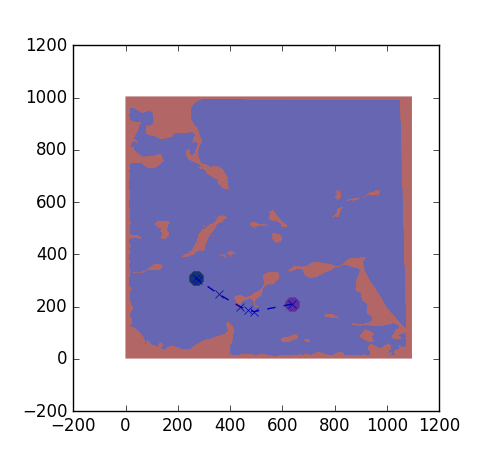
\includegraphics[width=\textwidth,trim={4cm 3cm 2cm 3cm},clip]{EXP3RG_PathCb_-1_-1_0_0.png}
        \caption[]{{\small Task 3-B, terrain only}}   
        \label{fig:Path_3-B_terrain}
    \end{subfigure}
    \vskip\baselineskip   
    
    \begin{subfigure}[b]{0.4\textwidth}
        \centering
        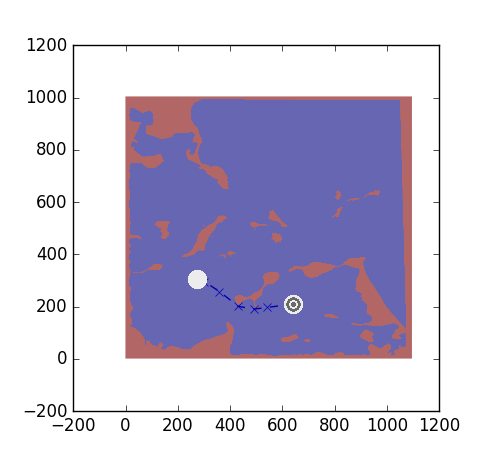
\includegraphics[width=\textwidth,trim={4cm 3cm 2cm 3cm},clip]{EXP3RG_PathCa_-1_-1_-1_0.png}
        \caption[]{{\small Task 3-A, terrain + work}}    
        \label{fig:Path_3-A_terrain_work}
    \end{subfigure}
    \hfill
    \begin{subfigure}[b]{0.4\textwidth}  
        \centering 
        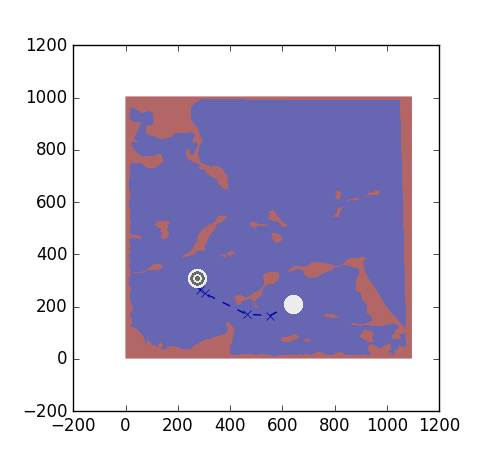
\includegraphics[width=\textwidth,trim={4cm 3cm 2cm 3cm},clip]{EXP3RG_PathCb_-1_-1_-1_0.png}
        \caption[]{{\small Task 3-B, terrain + work}}   
        \label{fig:Path_3-B_terrain_work}
    \end{subfigure}

    \begin{subfigure}[b]{0.4\textwidth}
        \centering
        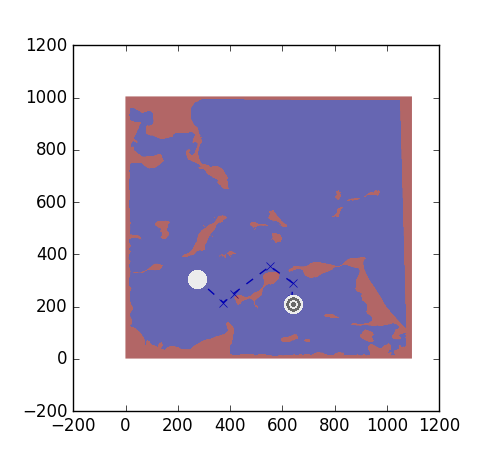
\includegraphics[width=\textwidth,trim={4cm 3cm 2cm 3cm},clip]{EXP3RG_PathCa_-1_-1_0_-1.png}
        \caption[]{{\small Task 3-A, terrain + reward}}    
        \label{fig:Path_3-A_terrain_reward}
    \end{subfigure}
    \hfill
    \begin{subfigure}[b]{0.4\textwidth}  
        \centering 
        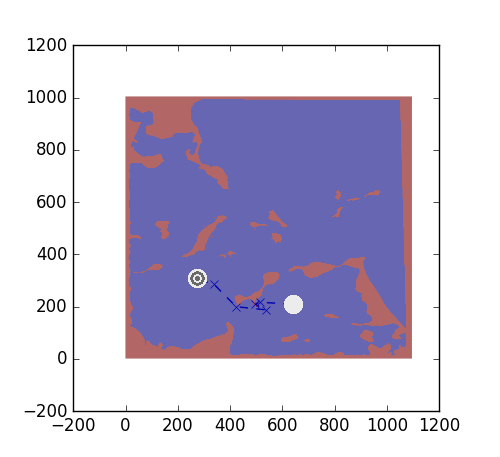
\includegraphics[width=\textwidth,trim={4cm 3cm 2cm 3cm},clip]{EXP3RG_PathCb_-1_-1_0_-1.png}
        \caption[]{{\small Task 3-B, terrain + reward}}   
        \label{fig:Path_3-B_terrain_reward}
    \end{subfigure}
    
  \begin{subfigure}[b]{0.4\textwidth}
        \centering
        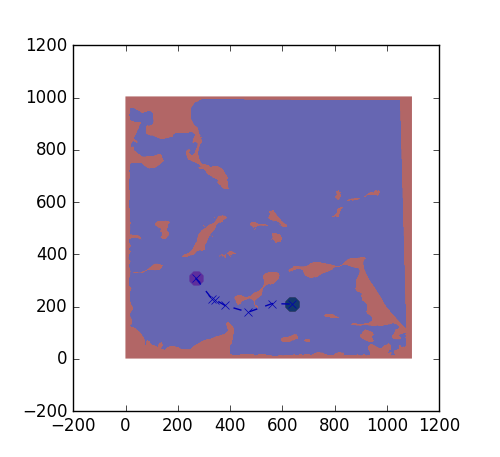
\includegraphics[width=\textwidth,trim={4cm 3cm 2cm 3cm},clip]{EXP3RG_PathCa_-1_-1_-1_-1.png}
        \caption[]{{\small Task 3-A, terrain + work + reward}}    
        \label{fig:Path_3-A_terrain_work_reward}
    \end{subfigure}
    \hfill
    \begin{subfigure}[b]{0.4\textwidth}  
        \centering 
        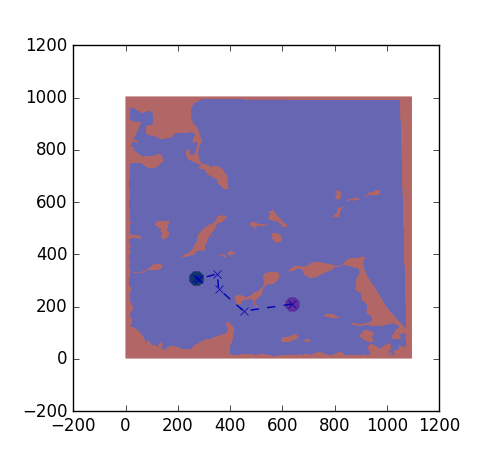
\includegraphics[width=\textwidth,trim={4cm 3cm 2cm 3cm},clip]{EXP3RG_PathCb_-1_-1_-1_-1.png}
        \caption[]{{\small Task 3-B, terrain + work + reward}}   
        \label{fig:Path_3-B_terrain_work_reward}
    \end{subfigure}

    \caption[]{\small Solution paths for tasks 3-A and 3-B, with and without work and reward concerns.} 
    \label{fig:Paths_3-A_3-B}
\end{figure*}
%%%%%%%%%%%%%%%%%%%%%%%%%%%%%%
%End Goto paths for 3-A, 3-B %
%%%%%%%%%%%%%%%%%%%%%%%%%%%%%%



%%%%%%%%%%%%%%%%%%%%%%%%%%%
% Goto paths for *-A, *-B %
%%%%%%%%%%%%%%%%%%%%%%%%%%%
\begin{figure*}
    \centering
    \begin{subfigure}[b]{0.24\textwidth}
        \centering
        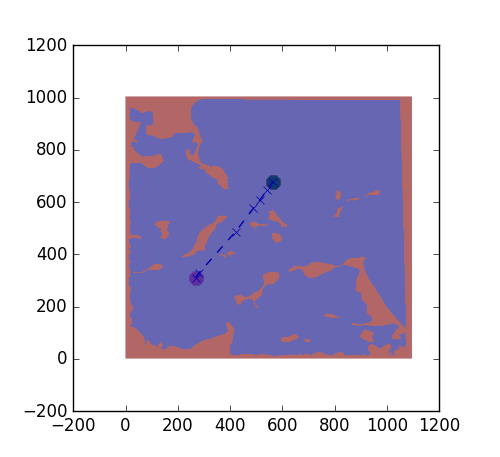
\includegraphics[width=\textwidth,trim={4cm 3cm 2cm 3cm},clip]{EXP3RG_PathAa_-1_-1_0d001_0.png}
        \caption[]{{\small Task 1-A \\ $W_{current}$: 0.001 \\ $W_{reward}$: 0}}    
        \label{fig:Path_1-A_upCurrent_noReward}
    \end{subfigure}
    \begin{subfigure}[b]{0.24\textwidth}  
        \centering 
        \includegraphics[width=\textwidth,trim={4cm 3cm 2cm 3cm},clip]{EXP3RG_PathAa_-1_-1_0d001_-1.png}
        \caption[interval 3]%
        {{\small Task 1-A \\ $W_{current}$: 0.001 \\ $W_{reward}$: 0.001}}
        \label{fig:Path_1-A_upCurrent_Reward}
    \end{subfigure}
    \begin{subfigure}[b]{0.24\textwidth}
        \centering
        \includegraphics[width=\textwidth,trim={4cm 3cm 2cm 3cm},clip]{EXP3RG_PathAb_-1_-1_0d001_0.png}
        \caption[interval 1]%
        {{\small Task 1-B \\ $W_{current}$: 0.001 \\ $W_{reward}$: 0}}
        \label{fig:Path_1-B_upCurrent_noReward}
    \end{subfigure}
    \begin{subfigure}[b]{0.24\textwidth}  
        \centering 
        \includegraphics[width=\textwidth,trim={4cm 3cm 2cm 3cm},clip]{EXP3RG_PathAb_-1_-1_0d001_-1.png}
        \caption[interval 3]%
        {{\small Task 1-B \\ $W_{current}$: 0.001 \\ $W_{reward}$: 0.001}}
        \label{fig:Path_1-B_upCurrent_Reward}
    \end{subfigure}
    
    \vskip\baselineskip  
        
    \begin{subfigure}[b]{0.24\textwidth}
        \centering
        \includegraphics[width=\textwidth,trim={4cm 3cm 2cm 3cm},clip]{EXP3RG_PathBa_-1_-1_0d001_0.png}
        \caption[interval 1]%
        {{\small Task 2-A \\ $W_{current}$: 0.001 \\ $W_{reward}$: 0}}    
        \label{fig:Path_2-A_upCurrent_noReward}
    \end{subfigure}
    \begin{subfigure}[b]{0.24\textwidth}  
        \centering 
        \includegraphics[width=\textwidth,trim={4cm 3cm 2cm 3cm},clip]{EXP3RG_PathBa_-1_-1_0d001_-1.png}
        \caption[interval 3]%
        {{\small Task 2-A \\ $W_{current}$: 0.001 \\ $W_{reward}$: 0.001}}   
        \label{fig:Path_2-A_upCurrent_Reward}
    \end{subfigure}
  \begin{subfigure}[b]{0.24\textwidth}
        \centering
        \includegraphics[width=\textwidth,trim={4cm 3cm 2cm 3cm},clip]{EXP3RG_PathBb_-1_-1_0d001_0.png}
        \caption[interval 1]%
        {{\small Task 2-B \\ $W_{current}$: 0.001 \\ $W_{reward}$: 0}}    
        \label{fig:Path_2-B_upCurrent_noReward}
    \end{subfigure}
    \begin{subfigure}[b]{0.24\textwidth}  
        \centering 
        \includegraphics[width=\textwidth,trim={4cm 3cm 2cm 3cm},clip]{EXP3RG_PathBb_-1_-1_0d001_-1.png}
        \caption[interval 3]%
        {{\small Task 2-B \\ $W_{current}$: 0.001 \\ $W_{reward}$: 0.001}}   
        \label{fig:Path_2-B_upCurrent_Reward}
    \end{subfigure}
    
    \vskip\baselineskip       

    \begin{subfigure}[b]{0.24\textwidth}
        \centering
        \includegraphics[width=\textwidth,trim={4cm 3cm 2cm 3cm},clip]{EXP3RG_PathCa_-1_-1_0d001_0.png}
        \caption[]{{\small Task 3-A \\ $W_{current}$: 0.001 \\ $W_{reward}$: 0}}    
        \label{fig:Path_3-A_upCurrent_noReward}
    \end{subfigure}
    \begin{subfigure}[b]{0.24\textwidth}  
        \centering 
        \includegraphics[width=\textwidth,trim={4cm 3cm 2cm 3cm},clip]{EXP3RG_PathCa_-1_-1_0d001_-1.png}
        \caption[]{{\small Task 3-A \\ $W_{current}$: 0.001 \\ $W_{reward}$: 0.001}}   
        \label{fig:Path_3-A_upCurrent_Reward}
    \end{subfigure}
    \begin{subfigure}[b]{0.24\textwidth}
        \centering
        \includegraphics[width=\textwidth,trim={4cm 3cm 2cm 3cm},clip]{EXP3RG_PathCb_-1_-1_0d001_0.png}
        \caption[]{{\small Task 3-B \\ $W_{current}$: 0.001 \\ $W_{reward}$: 0}}    
        \label{fig:Path_3-B_upCurrent_noReward}
    \end{subfigure}
    \begin{subfigure}[b]{0.24\textwidth}  
        \centering 
        \includegraphics[width=\textwidth,trim={4cm 3cm 2cm 3cm},clip]{EXP3RG_PathCb_-1_-1_0d001_-1.png}
        \caption[]{{\small Task 3-B \\ $W_{current}$: 0.001 \\ $W_{reward}$: 0.001}}   
        \label{fig:Path_3-B_upCurrent_Reward}
    \end{subfigure}
    \vskip\baselineskip      

    \caption[]{\small Solutions for Goto tasks, with increased $W_{current}$ and toggled $W_{reward}$.} 
    \label{fig:TestWorkWeight}
\end{figure*}

\begin{figure*}
    \centering
    \begin{subfigure}[b]{0.24\textwidth}
        \centering
            \includegraphics[width=\textwidth,trim={4cm 3cm 2cm 3cm},clip]{EXP3RG_PathAa_-1_-1_0_0d01.png}
        \caption[]{{\small Path 1-A \\ $W_{current}$: 0 \\ $W_{reward}$: 0.01}}    
        \label{fig:Path_1-A_upReward_noWork}
    \end{subfigure}
    %\hfill
    \begin{subfigure}[b]{0.24\textwidth}  
        \centering 
        \includegraphics[width=\textwidth,trim={4cm 3cm 2cm 3cm},clip]{EXP3RG_PathAa_-1_-1_-1_0d01.png}
        \caption[]{{\small Path 1-A \\ $W_{current}$: 0.00001 \\ $W_{reward}$: 0.01}}
        \label{fig:Path_1-A_upReward_Work}
    \end{subfigure}
    %\hfill
    \begin{subfigure}[b]{0.24\textwidth}
        \centering
        \includegraphics[width=\textwidth,trim={4cm 3cm 2cm 3cm},clip]{EXP3RG_PathAb_-1_-1_0_0d01.png}
        \caption[]{{\small Path 1-B \\ $W_{current}$: 0 \\ $W_{reward}$: 0.01}}
        \label{fig:Path_1-B_upReward_noWork}
    \end{subfigure}
    %\hfill
    \begin{subfigure}[b]{0.24\textwidth}  
        \centering 
        \includegraphics[width=\textwidth,trim={4cm 3cm 2cm 3cm},clip]{EXP3RG_PathAb_-1_-1_-1_0d01.png}
        \caption[]{{\small Path 1-B \\ $W_{current}$: 0.00001 \\ $W_{reward}$: 0.01}}
        \label{fig:Path_1-B_upReward_Work}
    \end{subfigure}
    
    \vskip\baselineskip  
        
    \begin{subfigure}[b]{0.24\textwidth}
        \centering
        \includegraphics[width=\textwidth,trim={4cm 3cm 2cm 3cm},clip]{EXP3RG_PathBa_-1_-1_0_0d01.png}
        \caption[]{{\small Path 2-A \\ $W_{current}$: 0 \\ $W_{reward}$: 0.01}}    
        \label{fig:Path_2-A_upReward_noWork}
    \end{subfigure}
    \begin{subfigure}[b]{0.24\textwidth}  
        \centering 
        \includegraphics[width=\textwidth,trim={4cm 3cm 2cm 3cm},clip]{EXP3RG_PathBa_-1_-1_-1_0d01.png}
        \caption[]{{\small Path 2-A \\ $W_{current}$: 0.00001 \\ $W_{reward}$: 0.01}}   
        \label{fig:Path_2-A_upReward_Work}
    \end{subfigure}
  \begin{subfigure}[b]{0.24\textwidth}
        \centering
        \includegraphics[width=\textwidth,trim={4cm 3cm 2cm 3cm},clip]{EXP3RG_PathBb_-1_-1_0_0d01.png}
        \caption[]{{\small Path 2-B \\ $W_{current}$: 0 \\ $W_{reward}$: 0.01}}    
        \label{fig:Path_2-B_upReward_noWork}
    \end{subfigure}
    \begin{subfigure}[b]{0.24\textwidth}  
        \centering 
        \includegraphics[width=\textwidth,trim={4cm 3cm 2cm 3cm},clip]{EXP3RG_PathBb_-1_-1_-1_0d01.png}
        \caption[]{{\small Path 2-B \\ $W_{current}$: 0.00001 \\ $W_{reward}$: 0.01}}   
        \label{fig:Path_2-B_upReward_Work}
    \end{subfigure}
    
    \vskip\baselineskip       

    \begin{subfigure}[b]{0.24\textwidth}
        \centering
            \includegraphics[width=\textwidth,trim={4cm 3cm 2cm 3cm},clip]{EXP3RG_PathCa_-1_-1_0_0d01.png}
        \caption[]{{\small Path 3-A \\ $W_{current}$: 0 \\ $W_{reward}$: 0.01}}    
        \label{fig:Path_3-A_upReward_noWork}
    \end{subfigure}
    \begin{subfigure}[b]{0.24\textwidth}  
        \centering 
        \includegraphics[width=\textwidth,trim={4cm 3cm 2cm 3cm},clip]{EXP3RG_PathCa_-1_-1_-1_0d01.png}
        \caption[]{{\small Path 3-A \\ $W_{current}$: 0.00001 \\ $W_{reward}$: 0.01}}   
        \label{fig:Path_3-A_upReward_Work}
    \end{subfigure}
    \begin{subfigure}[b]{0.24\textwidth}
        \centering
        \includegraphics[width=\textwidth,trim={4cm 3cm 2cm 3cm},clip]{EXP3RG_PathCb_-1_-1_0_0d01.png}
        \caption[]{{\small Path 3-B \\ $W_{current}$: 0 \\ $W_{reward}$: 0.01}}    
        \label{fig:Path_3-B_upReward_noWork}
    \end{subfigure}
    \begin{subfigure}[b]{0.24\textwidth}  
        \centering 
        \includegraphics[width=\textwidth,trim={4cm 3cm 2cm 3cm},clip]{EXP3RG_PathCb_-1_-1_-1_0d01.png}
        \caption[]{{\small Path 3-B \\ $W_{current}$: 0.00001 \\ $W_{reward}$: 0.01}}   
        \label{fig:Path_3-B_upReward_Work}
    \end{subfigure}
    \vskip\baselineskip      

    \caption[]{\small Solutions for Goto tasks, with increased $W_{reward}$ and toggled $W_{current}$.} 
    \label{fig:TestRewardWeight}
\end{figure*}


\begin{figure*}
    \centering
    \begin{subfigure}[b]{0.24\textwidth}
        \centering
            \includegraphics[width=\textwidth,trim={4cm 3cm 2cm 3cm},clip]{EXP3RG_PathAa_-1_-1_0d001_0d01.png}
        \caption[]{{\small Path 1-A \\ $W_{current}$: 0.001 \\ $W_{reward}$: 0.01}}    
        \label{fig:Path_1-A_upReward_upWork}
    \end{subfigure}
    %\hfill
    \begin{subfigure}[b]{0.24\textwidth}  
        \centering 
        \includegraphics[width=\textwidth,trim={4cm 3cm 2cm 3cm},clip]{EXP3RG_PathBa_-1_-1_0d001_0d01.png}
        \caption[]{{\small Path 2-A \\ $W_{current}$: 0.001 \\ $W_{reward}$: 0.01}}
        \label{fig:Path_2-A_upReward_upWork}
    \end{subfigure}
    %\hfill
    \begin{subfigure}[b]{0.24\textwidth}
        \centering
        \includegraphics[width=\textwidth,trim={4cm 3cm 2cm 3cm},clip]{EXP3RG_PathBa_-1_-1_0d001_0d01.png}
        \caption[]{{\small Path 2-A \\ $W_{current}$: 0.001 \\ $W_{reward}$: 0.01}}
        \label{fig:Path_3-A_upReward_upWork}
    \end{subfigure}
    
    \vskip\baselineskip  
        
    \begin{subfigure}[b]{0.24\textwidth}
        \centering
        \includegraphics[width=\textwidth,trim={4cm 3cm 2cm 3cm},clip]{EXP3RG_PathAb_-1_-1_0d001_0d01.png}
        \caption[]{{\small Path 1-B \\ $W_{current}$: 0.001 \\ $W_{reward}$: 0.01}}    
        \label{fig:Path_1-B_upReward_upWork}
    \end{subfigure}
    \begin{subfigure}[b]{0.24\textwidth}  
        \centering 
        \includegraphics[width=\textwidth,trim={4cm 3cm 2cm 3cm},clip]{EXP3RG_PathBb_-1_-1_0d001_0d01.png}
        \caption[]{{\small Path 2-B \\ $W_{current}$: 0.001 \\ $W_{reward}$: 0.01}}   
        \label{fig:Path_2-B_upReward_upWork}
    \end{subfigure}
  \begin{subfigure}[b]{0.24\textwidth}
        \centering
        \includegraphics[width=\textwidth,trim={4cm 3cm 2cm 3cm},clip]{EXP3RG_PathCb_-1_-1_0d001_0d01.png}
        \caption[]{{\small Path 3-B \\ $W_{current}$: 0.001 \\ $W_{reward}$: 0.01}}    
        \label{fig:Path_3-B_upReward_upWork}
    \end{subfigure}
    
    \vskip\baselineskip       
    
    \caption[]{\small Solutions for Goto tasks, with increased $W_{reward}$ and increased $W_{current}$.} 
    \label{fig:TestWorkRewardIncrease}
\end{figure*}


\begin{figure*}
    \centering
    \begin{subfigure}[b]{0.24\textwidth}
        \centering
            \includegraphics[width=\textwidth,trim={4cm 3cm 2cm 3cm},clip]{EXP3RG_PathAa_-1_-1_0d01_0d005.png}
        \caption[]{{\small Path 1-A \\ $W_{current}$: 0.01 \\ $W_{reward}$: 0.005}}    
        \label{fig:Path_1-A_upReward_upWork_b}
    \end{subfigure}
    %\hfill
    \begin{subfigure}[b]{0.24\textwidth}  
        \centering 
        \includegraphics[width=\textwidth,trim={4cm 3cm 2cm 3cm},clip]{EXP3RG_PathBa_-1_-1_0d01_0d005.png}
        \caption[]{{\small Path 2-A \\ $W_{current}$: 0.01 \\ $W_{reward}$: 0.005}}
        \label{fig:Path_2-A_upReward_upWork_b}
    \end{subfigure}
    %\hfill
    \begin{subfigure}[b]{0.24\textwidth}
        \centering
        \includegraphics[width=\textwidth,trim={4cm 3cm 2cm 3cm},clip]{EXP3RG_PathBa_-1_-1_0d01_0d005.png}
        \caption[]{{\small Path 2-A \\ $W_{current}$: 0.01 \\ $W_{reward}$: 0.005}}
        \label{fig:Path_3-A_upReward_upWork_b}
    \end{subfigure}
    
    \vskip\baselineskip  
        
    \begin{subfigure}[b]{0.24\textwidth}
        \centering
        \includegraphics[width=\textwidth,trim={4cm 3cm 2cm 3cm},clip]{EXP3RG_PathAb_-1_-1_0d01_0d005.png}
        \caption[]{{\small Path 1-B \\ $W_{current}$: 0.01 \\ $W_{reward}$: 0.005}}    
        \label{fig:Path_1-B_upReward_upWork_b}
    \end{subfigure}
    \begin{subfigure}[b]{0.24\textwidth}  
        \centering 
        \includegraphics[width=\textwidth,trim={4cm 3cm 2cm 3cm},clip]{EXP3RG_PathBb_-1_-1_0d01_0d005.png}
        \caption[]{{\small Path 2-B \\ $W_{current}$: 0.01 \\ $W_{reward}$: 0.005}}   
        \label{fig:Path_2-B_upReward_upWork_b}
    \end{subfigure}
  \begin{subfigure}[b]{0.24\textwidth}
        \centering
        \includegraphics[width=\textwidth,trim={4cm 3cm 2cm 3cm},clip]{EXP3RG_PathCb_-1_-1_0d01_0d005.png}
        \caption[]{{\small Path 3-B \\ $W_{current}$: 0.01 \\ $W_{reward}$: 0.005}}    
        \label{fig:Path_3-B_upReward_upWork_b}
    \end{subfigure}
    
    \vskip\baselineskip       
    
    \caption[]{\small Solutions for Goto tasks, with balance of increased $W_{reward}$ and increased $W_{current}$.} 
    \label{fig:TestWorkRewardIncreaseBalance}
\end{figure*}



%%%%%%%%%%%%%%%%%%%%%%%%%%%%%%
%End Goto paths for *-A, *-B %
%%%%%%%%%%%%%%%%%%%%%%%%%%%%%%


















\section{Coverage Planner}


\subsection{Region Without Terrain}

\singlespacing
\begin{table}[H]
    \begin{tabular}{lllllllllll}
 \thead{Region} & \thead{Region size \\ (meters)} & \thead{Region size \\ (cells)} & \thead{Current \\ complexity} & \thead{Distance \\ (meters)} & \thead{Duration \\ (minutes)} & \thead{Reward} & \thead{current updates}  \\
1 & 1450 & 10 x 10 & & 118.246 & 0.768 & 10643.620           & 0 \\
2 & 36250  & 50 x 50 & & 2598.042 & 16.870 & 407659.374      & 0 \\
3 & 145000 & 100 x 100 & & 10198.020 & 66.221 & 1030030.385  & 3 \\
4 & 326250 & 150 x 150 & & 22798.014 & 148.039 & 1926660.004 & 5 \\
5 & 580000 & 200 x 200 & & 40398.010 & 262.325 & 3520605.632 & 9
    \end{tabular}
\end{table}
\doublespacing

\singlespacing
\begin{table}[H]
    \begin{tabular}{lllllllllll}
\thead{Region} & \thead{Work columnwise \\ (with updates)} & \thead{Work rowwise \\ (with updates)}  & \thead{Work columnwise \\ (no updates} & \thead{Work rowwise \\ (no updates)} \\
1 &    513465.892 &    513452.073 & 513465.892 & 513452.073 &  \\
2 &  11903001.793 &  11890847.012 & 11903001.793 & 11890847.012 &   \\
3 &  47145978.158 &  47119054.520 & 47146078.734 & 47124199.557 &   \\
4 & 105728388.430 & 105685825.846 & 105704102.314 & 105728540.700  \\
5 & 187649992.045 & 187181080.951 & 187497561.286 & 187650706.827
    \end{tabular}
\end{table}
\doublespacing

\singlespacing
\begin{table}[H]
    \begin{tabular}{lllllllllll}
\thead{Region} & \thead{Work difference \\ (with updates)} & \thead{Work difference \\ (no updates} & \thead{Difference of differences \\ (updates or not)}  \\
1 &     13.819 & 13.819    & 0 \\
2 &  12154.781 & 12154.781 & 0 \\
3 &  26923.638 & 21879.177 & 5044.461  \\
4 &  42562.584 & 24438.386 & 18124.198  \\
5 & 468911.094 & 153145.541 & 315765.553
    \end{tabular}
\end{table}
\doublespacing

%%%%%%%%%%%%%%%%%%%%%%%%%
% Work coverage compare %
%%%%%%%%%%%%%%%%%%%%%%%%%

\begin{figure*}
    \captionsetup{justification=centering}
    \centering
    \begin{subfigure}[b]{0.275\textwidth}
        \centering
        \includegraphics[width=\textwidth]{work_r1.png}
        %\caption[]{{\small Convergence for particle swarm optimization}}
        \label{fig:coverage_noterrain_work_r1}
    \end{subfigure}
    \hfill
    \begin{subfigure}[b]{0.275\textwidth}  
        \centering 
        \includegraphics[width=\textwidth]{diff_r1.png}
        %\caption[]{{\small Convergence for bee colony optimization }}
        \label{fig:coverage_noterrain_work_diff_r1}
    \end{subfigure}
    \vskip\baselineskip
    \begin{subfigure}[b]{0.275\textwidth}
        \centering
        \includegraphics[width=\textwidth]{work_r2.png}
        %\caption[]{{\small Convergence for particle swarm optimization}}
        \label{fig:coverage_noterrain_work_r2}
    \end{subfigure}
    \hfill
    \begin{subfigure}[b]{0.275\textwidth}  
        \centering 
        \includegraphics[width=\textwidth]{diff_r2.png}
        %\caption[]{{\small Convergence for bee colony optimization }}
        \label{fig:coverage_noterrain_work_diff_r2}
    \end{subfigure}
    \vskip\baselineskip
    \begin{subfigure}[b]{0.275\textwidth}
        \centering
        \includegraphics[width=\textwidth]{work_r3.png}
        %\caption[]{{\small Convergence for particle swarm optimization}}
        \label{fig:coverage_noterrain_work_r3}
    \end{subfigure}
    \hfill
    \begin{subfigure}[b]{0.275\textwidth}  
        \centering 
        \includegraphics[width=\textwidth]{diff_r3.png}
        %\caption[]{{\small Convergence for bee colony optimization }}
        \label{fig:coverage_noterrain_work_diff_r3}
    \end{subfigure}
    \vskip\baselineskip
    \begin{subfigure}[b]{0.275\textwidth}
        \centering
        \includegraphics[width=\textwidth]{work_r4.png}
        %\caption[]{{\small Convergence for particle swarm optimization}}
        \label{fig:coverage_noterrain_work_r4}
    \end{subfigure}
    \hfill
    \begin{subfigure}[b]{0.275\textwidth}  
        \centering 
        \includegraphics[width=\textwidth]{diff_r4.png}
        %\caption[]{{\small Convergence for bee colony optimization }}
        \label{fig:coverage_noterrain_work_diff_r4}
    \end{subfigure}
    \vskip\baselineskip
    \begin{subfigure}[b]{0.275\textwidth}
        \centering
        \includegraphics[width=\textwidth]{work_r5.png}
        %\caption[]{{\small Convergence for particle swarm optimization}}
        \label{fig:coverage_noterrain_work_r5}
    \end{subfigure}
    \hfill
    \begin{subfigure}[b]{0.275\textwidth}  
        \centering 
        \includegraphics[width=\textwidth]{diff_r5.png}
        %\caption[]{{\small Convergence for bee colony optimization }}
        \label{fig:coverage_noterrain_work_diff_r5}
    \end{subfigure}
    
    \caption[]{\small Comparison of work estimates with row-wise and column-wise coverage schemes. Comparing with both static and dynamic water currents} 
    \label{fig:coverage_noterrain_work}
    
\end{figure*}


\chapter{Future Work}
%Future work falls into three stages. The first is straightforward, but necessary before introducing new features so that the system does not become unmanageable complex. The system is composed of numerous modules such as path planners, visualizations, report generators, and target selectors. While working on this thesis, data formats change, hard-coded data and paths are occasionally inserted, loops are executed in sequence that could be collapsed onto one, and other issues are present that impact both usability and performance. Code re-factoring and various small fixes are required to make the system user-friendly, accepting of more data sources, and generally improved. The mission planner should require very little interaction after initial setup, and should be accessible as part of a complete autonomous mobile robot.

%The second stage is to bridge the gap between a kinematic-based planner and dynamic USVs (real or simulated) using the solutions. 

%The major output of the mission planner is an ordered set of mission segments. Each segment has a path as a sequence of coordinates and estimates of the path's distance, duration, work, and reward. The coordinates are in latitude and longitude and thus immediately usable by GPS-based navigation systems (available on most USVs). However, the dynamics of real vehicles are such that the paths generated by a kinematic-based planner are unlikely to be optimal compared to one where the dynamics are taken into account. The path attribute estimates are idealized and will disagree with observations. Regardless of dynamics, a longer path that has to overcome stronger water currents will typically be worse than a shorter path on smoother seas. Thus, the planner results should be reasonable effective, especially the Goto paths. The coverage paths require a number of turns and are heavily impacted by the turning radius of the vehicle. Spiral paths are much more effective for a USV than a back-and-forth lawnmower path; it makes the most of the boat's turning radius instead of requiring it to slow down and turn. In this second stage, the goal is to ensure that the mission is feasible for a dynamic robot, rather than optimal. A method must be developed to use experiments to map a relationship between the planner's estimates and the duration, distance, and work observed in the field. This relationship can be used to generate a conservative constraint on the maximum duration and work so that the mission is feasible. This allows the underlying planners to remain generic and applicable to a variety of vehicles but still usable by a particular vehicle. 
%The shortest path to making this transition is to integrate the system with ROS. ROS is ... However, the current system is a set of perfectly usable programs and it should remain useful to non-ROS users. Thus, the system should have some intermediary module that, when online, makes the system both ROS-aware and ROS-accessible. This ROS-bridge module should suffice as the Navigator as far as this particular system goes so that it becomes useful to a wider robotics audience. This follows the ROS philosophy of.. 

%The third stage is to implement additional planning algorithms. These can be purely kinematic or parameterized on vehicle dynamics. The metaheuristic algorithms implemented so far have been shown to be effective, but all metaheuristic algorithms have a chance at failing or giving sub-optimal results. Having deterministic algorithms available can be useful if the computationally faster metaheuristics fail. Planners such as A*, D*, Voronoi diagram, rapidly-exploring random trees, graph-theory-based planners, among others, can be used for Goto planning. Coverage planning can be done in a variety of ways. Metaheuristic algorithms have difficulty with coverage when applied directly, but techniques exist to simplify the search space if the terrain is smoothed. Spiral or other geometric paths are ideal for USVs. An autonomous system should be flexible enough to handle a variety of situations and select the best planners for its environment and physical characteristics. 


\chapter{Conclusion}



\begin{appendices}
\chapter{Configuration File Examples}
\label{apx:config_files}

\begin{lstlisting}[language=bash, basicstyle=\small, label=lst:system_config, caption=Example system configuration file]
config:
    # Data Sources
    dataSources:
        # GeoTiff of the robot's mission region.
        regionRaster: "..../regionLand.tif"
        # NetCDF source of ocean forecasts. Used to get water currents.
        ncSourceURL: 'http://www.smast.umassd.edu:8080/thredds/dodsC/FVCOM/NECOFS/Forecasts/NECOFS_FVCOM_OCEAN_MASSBAY_FORECAST.nc'
        # GeoTiff of interpolated water current magnitude raster. Each band corresponds to time.
        currentsMagnitudeFile: "..../EXP3/SimuRaster_CurrentsMagnitude.tif"
        # Geotiff of interpolated water current direction raster. Each band corresponds to time.
        currentsDirectionFile: "..../SimuRaster_CurrentsDirection.tif"
        # Targets image file (may be set to None)
        targetsImg: "..../targets.png"
        # targets
        targetsTbl: "..../targets.csv" 
        # Target weights
        targetsWeights: "..../targetWeights.yaml"

    # Mission time frame and time resolution for forecast access. 
    missionTime:
        # Date (with time) to start the mission. 'None' will use current time. 
        startDate: None
        # Number of days to get forecasts for mission planning.
        numDays: 1
        # Interval (in minutes) resolution of forecasts to access.
        interval: 30

    # vehicle properties
    vehicle:
        # Mass of the vehicle in kilograms
        speed: 154 # in meters / minute
        # Position latitude (y)
        startCoordinates_lat: 42.2719 #42.5364
        # Position longitude (x)
        startCoordinates_lon: -70.9947 #-70.8786
        # Safepoints
        safepointsFile: "..../safepoints.csv"

    # Parameters for the Target Select path planner
    plannerTargetSelect:
        # Maximum number of targets to select
        maxSelect: 20
        # Pixel value that indicates land terrain (or other obstacle) in terrain raster.
        obstacleFlag: 1
        # Number of generations to evolve the optimization algorithm.
        generations: 1000
        # Number of individuals for optimization algorithm.
        individuals: 100

    # Parameters for the Goto path planner
    plannerGoto:
        # Number of waypoints for path. Note that dimension of problem equals numWaypoints * 2. 
        numWaypoints: 5
        # Pixel value that indicates land terrain (or other obstacle) in terrain raster.
        obstacle_flag: 1
        # Number of generations to evolve the optimization algorithm.
        generations: 10 #1000
        # Number of individuals for optimization algorithm.
        individuals: 10 #500
        # Distance weight (-1 for default)
        distanceWeight: -1
        # Obstacle weight (-1 for default)
        obstacleWeight: -1
        # Current weight (-1 for default)
        currentWeight: -1
        # Entity weight (-1 for default)
        entityWeight: -1

    # Parameters for the Coverage path planner
    plannerCoverage:
        # Number of generations to evolve the optimization algorithm
        generations: 100   
        # Number of individuals for optimization algorithm
        individuals: 100
        # Distance weight (-1 for default)
        distanceWeight: -1
        # Obstacle weight (-1 for default)
        obstacleWeight: -1
        # Skipped target weight (-1 for default)
        skipTargetWeight: -1
        # Energy expenditure (work) weight (-1 for default)
        workWeight: -1
        # Repeated node weight (-1 for default)
        repeatWeight: -1

    # Connection details for remote upload of results (set all to None if unused)
    ssh:
        # Server URI
        server: "....."
        # Server port
        port: 22
        # Username
        user: "ekrell"

    # Where, how to store output website
    output:
        # Prefix to organize runs
        prefix: "EXP3"
        # Should results be saved to remote server? (boolean)
        remote: True
        # Should results be saved as a local tar.gz? (boolean)
        archive: True
        # Path to output directory
        dir: "....."
        archivedir: "."
\end{lstlisting}


\begin{lstlisting}[language=bash, basicstyle=\small, label=lst:entities_config, caption=Example entities configuration file]
logbook:
    # Global weight. Significant of targets compared to other params
    tWeight: 10
    # Entities
    entities:
        - "T1"
        - "T2"
        - "T3"
        - "T4"
    # Weights on entity interest
    weights:
        - 1
        - 1
        - 1
        - 1
    weightDensity: 1
    weightSpeed: 1
    weightAcc: 1
    # Geotiff file names
    geotiffs:
        - "..../analyzed_T1.tiff"
        - "..../analyzed_T2.tiff"
        - "..../analyzed_T3.tiff"
        - "..../analyzed_T4.tiff"
    # Color code for the entities.
    # Uses the Red RGB value. Entities must have unique Red value. 
    # '255' already set aside as 'None' entity.
    colorcodes:
        0: 1    
        65: 3   
        225: 4  
        129: 2  
    targetDefaults:
        margin: 2
        roam: 0
\end{lstlisting}

\chapter{Experiment Result Tables}

\begin{small}
\begin{longtable}{lllllllllll}
\caption{Goto tasks, varying $W_{current}$ and $W_{reward}$}
    \label{Tbl:goto_weights} \\
\endfirsthead
\multicolumn{8}{c}{\tablename~\thetable\enspace(continued)}\\
\endhead
    \thead{Goto task} & \thead{$W_{work}$}  & \thead{$W_{reward}$} & \thead{Distance} 
            &  \thead{Duration}  & \thead{Work} & \thead{Reward}\\
    1-A &       0 &     0 & 471.923 & 3.064 &  872962.393 &  9656.377 \\
    1-A & 0.00001 &     0 & 471.948 & 3.065 &  872967.744 & 18777.098 \\
    1-A &       0 & 0.001 & 768.856 & 4.993 & 1636544.047 & 67658.128 \\
    1-A & 0.00001 & 0.001 & 763.616 & 4.958 & 1557155.114 & 67072.118 \\
    1-A & 0.001   &     0 &  472.162 &  3.066 &  873020.301 &  17717.608 \\
    1-A & 0.001   & 0.001 &  525.485 &  3.412 & 1020139.407 &  46335.398 \\
    1-A &     0   &  0.01 & 3450.169 & 22.404 & 7528778.003 & 187400.716 \\
    1-A & 0.00001 &  0.01 & 3553.073 & 23.072 & 7642390.213 & 184065.372 \\
    1-A & 0.001 &  0.01 & 2716.766 & 17.641 & 5690465.873 & 161057.493 \\
    1-A &  0.01 & 0.005 &  473.387 &  3.074 &  875326.291 &  19738.472 \\
    1-B &       0 &     0 & 471.931 & 3.065 &  874753.639 & 34380.806 \\
    1-B & 0.00001 &     0 & 476.249 & 3.093 &  898158.459 & 23764.245 \\
    1-B &       0 & 0.001 & 532.167 & 3.456 & 1138520.890 & 47056.326 \\
    1-B & 0.00001 & 0.001 & 523.406 & 3.399 & 1115227.670 & 46827.051 \\
    1-B & 0.001   &     0 &  472.688 &  3.069 &  877078.140 &  27233.786 \\
    1-B & 0.001   & 0.001 &  492.827 &  3.200 &  895667.841 &  39463.087 \\
    1-B &     0   &  0.01 & 3346.596 & 21.731 & 7426300.715 & 176643.009 \\
    1-B & 0.00001 &  0.01 & 3006.940 & 19.526 & 6646835.012 & 174816.752 \\
    1-B & 0.001 &  0.01 & 2323.835 & 15.090 & 5046559.944 & 157681.503 \\
    1-B &  0.01 & 0.005 &  480.604 &  3.121 &  877127.426 &  38241.258 \\
    2-A &         0 &   0 & 401.888 & 2.610 &  853713.591 & 38809.820 \\
    2-A & 0.00001 &     0 & 403.415 & 2.620 &  853732.981 & 37471.238 \\
    2-A &       0 & 0.001 & 522.720 & 3.394 & 1213325.807 & 60202.635 \\
    2-A & 0.00001 & 0.001 & 443.726 & 2.881 &  907456.347 & 48628.962 \\
    2-A & 0.001   &     0 &  398.038 &  2.585 &  853706.011 &  40290.358 \\
    2-A & 0.001   & 0.001 &  414.005 &  2.688 &  853737.973 &  42265.667 \\
    2-A &     0   &  0.01 & 2451.618 & 15.920 & 5470561.002 & 159071.320 \\
    2-A & 0.00001 &  0.01 & 2896.219 & 18.807 & 6508773.432 & 168811.209 \\
    2-A & 0.001 &  0.01 & 2924.143 & 18.988 & 6794756.462 & 177968.924 \\
    2-A &  0.01 & 0.005 &  432.643 &  2.810 &  853734.795 &  45290.396 \\
    2-B &       0 &     0 & 402.824 & 2.616 &  854046.146 & 26133.504 \\
    2-B & 0.00001 &     0 & 401.175 & 2.605 &  856286.108 & 31930.134 \\
    2-B &     0.0 & 0.001 & 534.978 & 3.474 & 1234339.173 & 78504.073 \\
    2-B & 0.00001 & 0.001 & 519.116 & 3.371 & 1152684.892 & 77127.633 \\
    2-B & 0.001   &     0 &  402.460 &  2.613 &  854040.946 &  26697.257 \\
    2-B & 0.001   & 0.001 &  471.576 &  3.062 &  961274.735 &  56279.423 \\
    2-B &     0   &  0.01 & 3454.049 & 22.429 & 7893027.478 & 207350.852 \\
    2-B & 0.00001 &  0.01 & 3138.368 & 20.379 & 6996373.723 & 195758.929 \\
    2-B & 0.001 &  0.01 & 2367.599 & 15.374 & 5372982.897 & 177593.131 \\
    2-B &  0.01 & 0.005 &  458.052 &  2.974 &  853940.514 &  55040.808 \\
    3-A &       0 &     0 & 414.048 & 2.689 &  884220.973 & 28662.233 \\
    3-A & 0.00001 &     0 & 403.967 & 2.623 &  872563.881 & 40112.844 \\
    3-A &       0 & 0.001 & 557.149 & 3.618 & 1068842.638 & 62362.396 \\
    3-A & 0.00001 & 0.001 & 422.454 & 2.743 &  912240.714 & 59076.483 \\
    3-A & 0.001   &     0 &  421.795 &  2.739 &  872536.380 &  38057.778 \\
    3-A & 0.001   & 0.001 &  514.209 &  3.339 & 1028936.298 &  18726.627 \\
    3-A &     0   &  0.01 & 3265.082 & 21.202 & 6949330.005 & 146020.149 \\
    3-A & 0.00001 &  0.01 & 2725.074 & 17.695 & 5930036.872 & 136888.759 \\
    3-A & 0.001 &  0.01 & 1073.221 & 6.969 & 2440013.221 & 110011.867 \\
    3-A &  0.01 & 0.005 &  441.574 & 2.867 &  872727.680 &  47660.029 \\
    3-B &       0 &     0 & 406.864 & 2.642 &  872543.353 & 12801.378 \\
    3-B & 0.00001 &     0 & 439.822 & 2.856 &  956466.487 & 12415.401 \\
    3-B &       0 & 0.001 & 495.576 & 3.218 & 1061702.130 & 40058.201 \\
    3-B & 0.00001 & 0.001 & 458.914 & 2.980 &  996343.932 & 26384.526 \\
    3-B & 0.001   &     0 &  468.168 &  3.040 &  937853.211 &  17361.288 \\
    3-B & 0.001   & 0.001 &  484.693 &  3.147 &  986881.612 &  34759.438 \\
    3-B &     0   &  0.01 & 3685.961 & 23.935 & 8291295.995 & 164667.291 \\
    3-B & 0.00001 &  0.01 & 3500.646 & 22.731 & 7921721.451 & 150845.048 \\
    3-B & 0.001 &  0.01 & 1648.077 & 10.70 & 3544961.693 & 98591.959 \\
    3-B &  0.01 & 0.005 &  421.438 &  2.737 & 872541.791 & 38134.278 \\      
\end{longtable}
\end{small}


\begin{small}
\begin{longtable}{lllllll}
\caption{Goto tasks using PSO, DE, SGA, and BEE}
    \label{Tbl:goto_algorithms}\\
 \endfirsthead
\multicolumn{7}{c}{\tablename~\thetable\enspace(continued)}\\
 \endhead
Algorithm & Optimizing & Run & Distance      & Duration      & Work          & Reward        \\
BEE & distance    & 1   & 455.071  & 2.96 & 961416.957 & 29450.317 \\
BEE & distance    & 2   & 404.815 & 2.629 & 854031.787 & 28672.502  \\
BEE & distance    & 3   & 419.943 & 2.727 & 898359.444 & 23597.349 \\
BEE & distance    & 4   & 479.542 & 3.114 & 991686.596 & 28661.570 \\
BEE & distance    & 5   & 420.851 & 2.733 & 870274.384 & 42033.125 \\
BEE & distance    & 6   & 426.629 & 2.770 & 886652.549 & 32240.980 \\
BEE & distance    & 7   & 407.363 & 2.645 & 853930.939 & 45735.287 \\
BEE & distance    & 8   & 432.098 & 2.806 & 903059.447 & 22193.102 \\
BEE & distance    & 9   & 407.363 & 2.645 & 853930.939 & 45735.287 \\
BEE & distance    & 10  & 405.377 & 2.632 & 854031.638 & 26375.820 \\
BEE & distance,work,reward & 1   & 413.181 & 2.680 & 853930.945 & 43815.927 \\
BEE & distance,work,reward & 2   & 492.752 & 3.200 & 931109.877 & 47693.685 \\
BEE & distance,work,reward & 3   & 547.830 & 3.557  & 1131765.593 & 70388.875  \\
BEE & distance,work,reward & 4   & 475.58 & 3.088 & 886653.266 & 36432.077 \\
BEE & distance,work,reward & 5   & 490.149 & 3.183 & 954350.373 & 51865.611 \\
BEE & distance,work,reward & 6   & 437.303 & 2.840 & 853970.171 & 49871.084 \\
BEE & distance,work,reward & 7   & 450.332 & 2.924 & 924201.879  & 22973.243  \\
BEE & distance,work,reward & 8   & 435.792 & 2.830 & 854087.083  & 35309.669 \\
BEE & distance,work,reward & 9   & 449.796 & 2.921 & 853948.539 & 30940.914 \\
BEE & distance,work,reward & 10  & 449.169 & 2.917 & 900744.74149  & 30226.910 \\
PSO & distance    & 1   & 401.957 & 2.610  & 853938.583 & 26350.350 \\
PSO & distance    & 2   & 401.592  & 2.608 & 856268.399 & 31325.840 \\
PSO & distance    & 3   & 404.669 & 2.628 & 861063.917 & 25458.829 \\
PSO & distance    & 4   & 420.305  & 2.729 & 877421.425 & 24586.357 \\
PSO & distance    & 5   & 405.908 & 2.636 & 856377.409 & 25893.182 \\
PSO & distance    & 6   & 401.433 & 2.607 & 854046.053 & 25910.487  \\
PSO & distance    & 7   & 398.148 & 2.585 & 853970.984 & 27693.397 \\
PSO & distance    & 8   & 405.908 & 2.636 & 856377.409 & 25893.182 \\
PSO & distance    & 9   & 405.032 & 2.630 & 854041.400  & 25620.923 \\
PSO & distance    & 10  & 403.116 & 2.618 & 854045.949 & 26075.484 \\
PSO & distance,work,reward    & 1   & 467.179 & 3.034 & 909915.488 & 50037.678 \\
PSO & distance,work,reward    & 2   & 442.047 & 2.870 & 863352.364 & 50011.205 \\
PSO & distance,work,reward    & 3   & 411.304 & 2.671 & 854048.792 & 27821.990 \\
PSO & distance,work,reward    & 6   & 441.674 & 2.868 & 860929.179 & 55359.840 \\
PSO & distance,work,reward    & 7   & 450.077 & 2.923 & 860978.180 & 43937.208 \\
PSO & distance,work,reward    & 8   & 462.366 & 3.002 & 853931.796 & 53048.567 \\
PSO & distance,work,reward    & 9   & 411.946 & 2.675 & 853961.433 & 41984.573 \\
PSO & distance,work,reward    & 10  & 502.618 & 3.264 & 926276.271 & 58267.140 \\
DE  & distance    & 1   & 547.457 & 3.555 & 1190088.188 & 31128.400 \\
DE  & distance    & 2   & 654.539 & 4.250 & 1409311.212 & 31003.023 \\
DE  & distance    & 3   & 657.115 & 4.267 & 1355924.052 & 22856.085 \\
DE  & distance    & 4   & 618.772 & 4.018 & 1367427.128 & 22832.142 \\
DE  & distance    & 5   & 600.323 & 3.898 & 1344186.805 & 32974.095 \\
DE  & distance    & 6   & 617.654 & 4.011 & 1253138.776 & 25312.875 \\
DE  & distance    & 7   & 601.219 & 3.904 & 1297328.352 & 53851.804 \\
DE  & distance    & 8   & 515.227 & 3.346 & 1059421.898 & 36982.003 \\
DE  & distance    & 9   & 621.422 & 4.035 & 1376866.439 & 36122.223 \\
DE  & distance    & 10  & 738.152 & 4.793 & 1540225.585 & 30053.169 \\
DE  & distance,work,reward  & 1  & 443.852 & 2.882 & 902948.385  & 45557.570 \\
DE  & distance,work,reward  & 2  & 499.009 & 3.240 & 1036000.476 & 32797.715 \\
DE  & distance,work,reward  & 3  & 598.428 & 3.886 & 1271818.341 & 34275.877 \\
DE  & distance,work,reward  & 4  & 547.222 & 3.553 & 1173566.823 & 31771.260 \\
DE  & distance,work,reward  & 5  & 569.007 & 3.695 & 1106033.136 & 52980.788 \\
DE  & distance,work,reward  & 6  & 560.045 & 3.637 & 1134183.095 & 29567.272 \\
DE  & distance,work,reward  & 7  & 499.009 & 3.240 & 1036000.476 & 32797.715 \\
DE  & distance,work,reward  & 8  & 603.100 & 3.916 & 1245992.043 & 48937.410 \\
DE  & distance,work,reward  & 9  & 513.718 & 3.336 & 1101439.368 & 31308.760 \\
DE  & distance,work,reward  & 10 & 437.116 & 2.838 &  860982.652 & 25451.409 \\
SGA & distance    & 1   & 547.457 & 3.555 & 1190088.188 & 31128.400 \\
SGA & distance    & 2   & 654.539 & 4.250 & 1409311.212 & 31003.023  \\
SGA & distance    & 3   & 657.115 & 4.267 & 1355924.052 & 22856.085 \\
SGA & distance    & 4   & 618.772 & 4.018 & 1367427.128 & 22832.142 \\
SGA & distance    & 5   & 600.323 & 3.898 & 1344186.805 & 32974.095 \\
SGA & distance    & 6   & 617.654 & 4.010 & 1253138.776 & 25312.875 \\
SGA & distance    & 7   & 601.219 & 3.904 & 1297328.352 & 53851.804 \\
SGA & distance    & 8   & 515.227 & 3.346 & 1059421.898 & 36982.003 \\
SGA & distance    & 9   & 621.422 & 4.035 & 1376866.439 & 36122.224 \\
SGA & distance    & 10  & 738.152 & 4.793 & 1540225.585 & 30053.169  \\
SGA & distance,work,reward    & 1   & 443.852 & 2.882 &  902948.385 & 45557.570 \\
SGA & distance,work,reward    & 2   & 499.009 & 3.240 & 1036000.476 & 32797.715 \\
SGA & distance,work,reward    & 3   & 598.428 & 3.886 & 1271818.341 & 34275.877 \\
SGA & distance,work,reward    & 4   & 547.222 & 3.553 & 1173566.823 & 31771.260 \\
SGA & distance,work,reward    & 5   & 569.007 & 3.694 & 1106033.138 & 52980.788 \\
SGA & distance,work,reward    & 6   & 560.045 & 3.637 & 1134183.095 & 29567.272 \\
SGA & distance,work,reward    & 7   & 499.009 & 3.240 & 1036000.476 & 32797.715 \\
SGA & distance,work,reward    & 8   & 603.100 & 3.916 & 1245992.043 & 48937.410 \\
SGA & distance,work,reward    & 9   & 513.718 & 3.336 & 1101439.368 & 31308.764 \\
SGA & distance,work,reward    & 10  & 437.116 & 2.838 &  860982.652 & 25451.409
\end{longtable}
\end{small}


\end{appendices}

\end{document}
